\documentclass{report}

% simple paragraph stuff
\parindent=0pt
\parskip=6pt

% include \paragraph as numbered
\setcounter{secnumdepth}{3}
\setcounter{tocdepth}{3}

% symbols
\usepackage{amsmath} % assumes amsmath package installed
\usepackage{amssymb} % for \square

% algorithm stuff
\usepackage{algorithm}
\usepackage[noend]{algpseudocode}

% theorems
\newtheorem{invariant}{Invariant}
\newtheorem{theorem}{Theorem}
\newtheorem{proposition}{Proposition}
\newtheorem{lemma}{Lemma}
% from http://www.maths.tcd.ie/~dwilkins/LaTeXPrimer/Theorems.html
\newenvironment{proof}[1][Proof]{\begin{trivlist}
   \item[\hskip \labelsep {\bfseries #1}]}{\hfill$\square$\end{trivlist}}

\usepackage{array}
\usepackage{graphicx}
\usepackage{subcaption}

\usepackage{tikz}
\usetikzlibrary{arrows,backgrounds,positioning,shapes,decorations.pathmorphing}

% plots
\usepackage{pgfplots}

\title{Fast Manipulation\\Task Planning}
\author{Christopher M. Dellin}
\date{\today} 

\begin{document}

\maketitle

\begin{abstract}
   Driven by a symbolic task planner, plan a feasible or low-cost sequence of
   robot trajectory segments to solve a multi-step manipulation problem
   (e.g. move an object, turn a valve, etc).
\end{abstract}

\tableofcontents


\newpage
\chapter{Introduction}

\section{Motivation}

\subsection{DRC}

Cite ISER paper \cite{dellin2014drc}.
Also the journal paper \cite{stentz2014chimp}.

\subsection{Speed! Minimize total task time}

How can we speed things up?

\subsection{Multiple steps, don't get stuck}

How can we keep from getting stuck?

\subsection{Changing environments}

\section{Approach}

Overview of approach.


\newpage
\chapter{Problem Description and Approach}
\label{chap:formulation}

\section{Multiple steps}

\subsection{steps from a human (drc) or symbolic planner}
\subsection{some steps are constrained}
\subsection{dual arm stuff}
\subsection{Different spaces}

multi-step problem structure (lots of options at each step)

decomposition into a bunch of "local planner" like things

\section{Approach}

Decompose the problem into multiple steps.
We'll build a meta-graph.

\section{Expensive checking}

\section{Dont't get stuck}

\section{Most queries will be unexecuted (opt later)}

\section{Approach}

Two complementary things:
make each step fast (Chapter~\ref{chap:inflate}),
and exploit structure between steps (Chapter~\ref{chap:multispace}).

Then we talk about the full task planner later.


\newpage
\chapter{Quickly Searching Manipulation Graphs}
\label{chap:inflate}

In order for an articulated robot to perform manipulation tasks
in changing, unstructured environments,
it must be able to quickly solve motion planning queries in its
configuration space.
While there are many types of approaches for such queries
which we discuss in Section~\ref{sec:related-work},
one of the most common are graph search algorithms.
In this chapter,
we discuss the efficiency tradeoffs induced by formulating
the articulated motion planning problem as best-first search,
propose a general planning framework which accounts for these tradeoffs,
and examine some empirical results.

\paragraph{Two Notions of Efficiency}

Throughout this chapter,
we reference two different types of efficiency
with regard to robotic tasks.
First, once a planner has computed a solution path or trajectory,
there is the cost incurred while executing that trajectory.
This is the traditional cost optimized for by planners.
Second, there is the cost incurred from actually computing the solution
itself.

This dichotomy of effort is, of course, not new.
From Winston's \emph{Articifial Intelligence} \cite{winston1977ai},
\begin{quote}
   ``Properly speaking, the problem of determining a good path is a search
   problem in which two kinds of effort are involved:
   \begin{itemize}
   \item First, there is the effort expended in \emph{finding} either
      some path or the best path.
   \item And, second, there is the effor actually expended in
      \emph{traversing} the network.''
   \end{itemize}
\end{quote}

For the application of manipulation planning for articulated robots,
in paricular,
the costs associated with these two components tend to be of comparable
magnitude.
For example,
when time is used as an efficency metric,
both planning and execution times for household applications
tend to be on the order of 1-2 seconds.
Alternatively, given
modern computational and actuator technologies for human-scale problems,
both planning and execution tend to consume similar amounts of energy.
Therefore,
the manipulation problem demands that
(a) the cost of plans and
(b) the cost of planning both be considered.

\paragraph{General Problem Characterization}

We are motivated to solve motion planning problems for articulated robots.
In the simplest version of this problem,
the robot has a continuous configuration space $C$,
with some subset $C_{obs}$ in collision.
All feasible trajectories must then lie entirely in
$C_{free} = C \setminus C_{obs}$.
In general, testing some configuration $q$ for membership in $C_{free}$
is an expensive operation.
A typical query asks for a trajectory $t: [0,1] \rightarrow Q$ between
a start set and a goal set (e.g. $t(0) \in Q_s$ and $t(1) \in Q_g$.
We defer discussion constraints until Section~\ref{sec:constraints}.
We are focused on configuration spaces without dynamics.

In this chapter,
we'll primarly focus on single-query things,
but we'll keep in mind that we want things that can enable reuse eventually.

While we will primarily apply graph search techniques to this problem,
we start by reviewing alternative approaches.

\section{Review of Alternative Approaches}
\label{sec:related-work}

Since $C$ is continuous,
all approaches must introduce some sort of discretization
in order to compute solutions.
We choose to build a graph consisting of vertices and edges in $C$,
and then search that graph (Section~\ref{sec:best-first}).
We do this because we can rely on existing techniques,
and because an explicit graph can be more easily reused than other
approaches.
In this section, we discuss alternative approaches to solving
the motion planning problem for articulated robots.

\subsection{Trajectory Optimization}

One approach is trajectory optimization.
For example, there's CHOMP \cite{zucker2013chomp}
and TrajOpt \cite{schulman2013trajopt}.
Lots of other prior work here that is not manipulation-focused.

Local minima problems.
Difficult to cache / apply to similar problems.

\subsection{Incremental Construction Algorithms}

We could construct the graph incrementally and in response to the shape
of $C_{free}$.
RRTs behave well for quickly finding feasible paths.
We'll compare against them at the end of this chapter.
Also talk about ESTs.
Difficult to cache things.

%\subsection{Multi-Query Approaches}
%
%We could run a PRM \cite{kavrakietal1996prm}.
%Commit to a fixed graph,
%and determine the validity of each vertex and edge w.r.t. $C_{free}$.
%Then, at query time,
%run A* to find the shortest path (this is fast due to graph sparseness).
%This is good because it reuses work.
%Unfortunately,
%(a) our $C_{free}$ is different for every subplan
%(and for different options with each),
%and (b) we don't want to determine validity over the entire graph
%because it's costly.

\subsection{Anytime algorithms}

Compare to RRT*, FMT*, BIT*, etc.

\section{Best-First Graph Search}
\label{sec:best-first}

In this section,
we discuss general best-first search over explicit graphs.

\subsection{Formulating Motion Planning as Graph Search}

Continuous space, graph over it.
We have a graph $G$ with vertices $V$ and edges $E$.
We have some start set $V_s$ and some goal set $V_g$.
We represent a path through the graph as
$\pi = \{ v_0, v_1, v_2, \dots, v_n \}$;
a candidate solution path then has $v_0 \in V_s$ and $v_n \in V_g$.
We assume that only edges have costs,
such that the cost of a path is the cost if its constituent edges.
The cost of an edge is given by $c(v_a,v_b)$, and is always non-negative.
We assume that the graph is endowed with an admissible heuristic edge cost
function
$\hat{c}(v_a,v_b)$
which is inexpensive to compute.

We observe that such graphs motion planning for articulated robots
exhibit several properties that influence solution techniques.

\textbf{Sparsity.}
The size of a graph necessary to solve common problems
is relatively small.
In particular, it is reasonable to store the entire graph explicitly in
memory;
techniques to incrementally build the graph
are not necessary.
Also,
we are not restricted to only expanding successors of a vertex;
we can simply make queries of the graph.
[NOTE: sparsity is not a good word here, since it already has meaning
for graphs.]

\textbf{Expensive Edge Evaluations.}
Evaluating edge costs (e.g. testing for membership in $C_{free}$)
is expensive.

See Figure~\ref{fig:seg-intro} for an example.

\begin{figure}
\centering
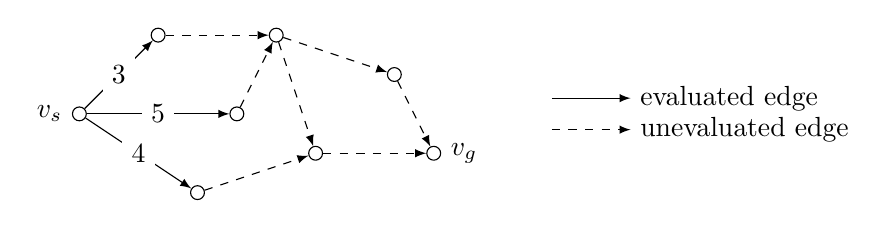
\begin{tikzpicture}
\tikzstyle{vertex}=[circle,draw=black,inner sep=0pt,minimum size=5pt]

\node[vertex] (a) at (0,0) {};
\node[vertex] (b) at (2,0) {};
\node[vertex] (c) at (2.5,1) {};
\node[vertex] (d) at (1,1) {};
\node[vertex] (e) at (3,-0.5) {};
\node[vertex] (f) at (4,0.5) {};
\node[vertex] (g) at (4.5,-0.5) {};
\node[vertex] (h) at (1.5,-1) {};

\draw[black,->,>=latex] (a) -- (b) node [midway, fill=white] {5};
\draw[black,->,>=latex] (a) -- (h) node [midway, fill=white] {4};
\draw[black,->,>=latex] (a) -- (d) node [midway, fill=white] {3};
\draw[black,->,dashed,>=latex] (b) -- (c);
\draw[black,->,dashed,>=latex] (d) -- (c);
\draw[black,->,dashed,>=latex] (c) -- (e);
\draw[black,->,dashed,>=latex] (c) -- (f);
\draw[black,->,dashed,>=latex] (f) -- (g);
\draw[black,->,dashed,>=latex] (e) -- (g);
\draw[black,->,dashed,>=latex] (h) -- (e);

\draw[black,->,>=latex] (6,0.2) -- (7,0.2);
\node[anchor=west] at (7,0.2) {evaluated edge};
\draw[black,->,dashed,>=latex] (6,-0.2) -- (7,-0.2);
\node[anchor=west] at (7,-0.2) {unevaluated edge};

\node[left=0pt of a] {$v_s$};
\node[right=0pt of g] {$v_g$};

\end{tikzpicture}
\caption{A small explicit graph with some evaluated edges.}
\label{fig:seg-intro}
\end{figure}

\subsection{Generic Best-First Search Algorithm over Paths}

Best-first search \cite{winston1977ai}
is a general class of search algorithms.
We choose to express the general algorith
over \emph{paths} instead of \emph{vertices}
for clarity and generality
because we are focused primarily on explicit graphs.
However, Section~\ref{sec:implicit} shows
how it reduces to traditional A* search
for certain types of evaluation functions,
as is required when searching over implicit graphs.

\begin{algorithm}
\caption{Generic Best-First Search Algorithm}
\label{alg:generic-best-first}
\begin{algorithmic}[1]
\Procedure {\textsc{GenericBestFirst}}{$G$}
\Loop
   \State $\pi^* = \arg \min\limits_{\Pi} f(\pi)$
      \Comment{For some path cost function $f(\pi)$}
      \label{line:select-optimistic-path}
   \If {$\pi^*$ fully evaluated}
      \State \Return $\pi^*$
   \EndIf
   \State \textsc{Evaluate}$(\pi^*)$
      \Comment{For some evaluate function}
\EndLoop
\EndProcedure
\end{algorithmic}
\end{algorithm}

Consider the general best-first search algorithm
(Algorithm~\ref{alg:generic-best-first}).
It maintains some sort of data structure storing known data about the
graph (e.g. tags on vertices or edges).
It simply iterates over optimistically-optimal ``best'' paths,
partially evaluating each.
(Note especially the greedy nature of this search.)
See Figure~\ref{fig:seg-edge-example} for a simple example.

\begin{figure}
\centering
\begin{subfigure}[b]{0.45\textwidth}
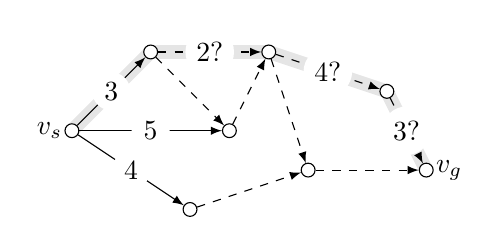
\begin{tikzpicture}
\tikzstyle{vertex}=[circle,draw=black,fill=white,inner sep=0pt,minimum size=5pt]

\coordinate (a) at (0,0);
\coordinate (b) at (2,0);
\coordinate (c) at (2.5,1);
\coordinate (d) at (1,1);
\coordinate (e) at (3,-0.5);
\coordinate (f) at (4,0.5);
\coordinate (g) at (4.5,-0.5);
\coordinate (h) at (1.5,-1);

\draw[black!10,line width=5pt,line cap=round] (a) -- (d) -- (c) -- (f) -- (g);

\node[vertex] (na) at (a) {};
\node[vertex] (nb) at (b) {};
\node[vertex] (nc) at (c) {};
\node[vertex] (nd) at (d) {};
\node[vertex] (ne) at (e) {};
\node[vertex] (nf) at (f) {};
\node[vertex] (ng) at (g) {};
\node[vertex] (nh) at (h) {};

\draw[black,->,>=latex] (na) -- (nb) node [circle,inner sep=2pt,midway,fill=white] {5};
\draw[black,->,>=latex] (na) -- (nh) node [circle,inner sep=2pt,midway,fill=white] {4};
\draw[black,->,>=latex] (na) -- (nd) node [circle,inner sep=2pt,midway,fill=white] {3};
\draw[black,->,dashed,>=latex] (nd) -- (nb);
\draw[black,->,dashed,>=latex] (nb) -- (nc);
\draw[black,->,dashed,>=latex] (nd) -- (nc) node [circle,inner sep=2pt,midway,fill=white] {2?};
\draw[black,->,dashed,>=latex] (nc) -- (ne);
\draw[black,->,dashed,>=latex] (nc) -- (nf) node [circle,inner sep=2pt,midway,fill=white] {4?};
\draw[black,->,dashed,>=latex] (nf) -- (ng) node [circle,inner sep=2pt,midway,fill=white] {3?};
\draw[black,->,dashed,>=latex] (ne) -- (ng);
\draw[black,->,dashed,>=latex] (nh) -- (ne);

\node[left=0pt of a] {$v_s$};
\node[right=0pt of g] {$v_g$};

\end{tikzpicture}
\caption{Select optimistic best path}
\end{subfigure}%
\quad%
\begin{subfigure}[b]{0.45\textwidth}
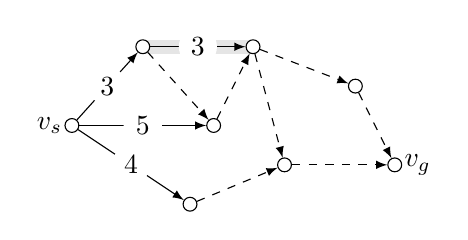
\begin{tikzpicture}
\tikzstyle{vertex}=[circle,draw=black,fill=white,inner sep=0pt,minimum size=5pt]

\coordinate (a) at (0,0);
\coordinate (b) at (1.8,0);
\coordinate (c) at (2.3,1);
\coordinate (d) at (0.9,1);
\coordinate (e) at (2.7,-0.5);
\coordinate (f) at (3.6,0.5);
\coordinate (g) at (4.1,-0.5);
\coordinate (h) at (1.5,-1);

\draw[black!10,line width=5pt,line cap=round] (d) -- (c);

\node[vertex] (na) at (a) {};
\node[vertex] (nb) at (b) {};
\node[vertex] (nc) at (c) {};
\node[vertex] (nd) at (d) {};
\node[vertex] (ne) at (e) {};
\node[vertex] (nf) at (f) {};
\node[vertex] (ng) at (g) {};
\node[vertex] (nh) at (h) {};

\draw[black,->,>=latex] (na) -- (nb) node [circle,inner sep=2pt,midway,fill=white] {5};
\draw[black,->,>=latex] (na) -- (nh) node [circle,inner sep=2pt,midway,fill=white] {4};
\draw[black,->,>=latex] (na) -- (nd) node [circle,inner sep=2pt,midway,fill=white] {3};
\draw[black,->,dashed,>=latex] (nd) -- (nb);
\draw[black,->,dashed,>=latex] (nb) -- (nc);
\draw[black,->,>=latex] (nd) -- (nc) node [circle,inner sep=2pt,midway,fill=white] {3};
\draw[black,->,dashed,>=latex] (nc) -- (ne);
\draw[black,->,dashed,>=latex] (nc) -- (nf);
\draw[black,->,dashed,>=latex] (nf) -- (ng);
\draw[black,->,dashed,>=latex] (ne) -- (ng);
\draw[black,->,dashed,>=latex] (nh) -- (ne);

\node[left=0pt of a] {$v_s$};
\node[right=0pt of g] {$v_g$};

\end{tikzpicture}
\caption{Evaluate first unevaluated edge}
\end{subfigure}%
\caption{Generic best-first algorithm for an explicit graph,
   with $f(\pi)$ best known cost-from-start,
   and {\sc Eval} forward edge evaluations.
   This algorithm is guaranteed to terminate with a feasible path
   with mimimum path cost, if one exists.}
\label{fig:seg-edge-example}
\end{figure}

There are two choices:

\textbf{Cost Function $f(\pi)$.}
What is the cost function $f(\pi)$ over paths used to select the
path for evaluation at each iteration?
For now, we will use the following path objective:
\begin{equation}
   f_x(\pi) = \mbox{\emph{optimistic estimate of execution effort}}.
\end{equation}
In other worts, $f_x(\pi)$ gives a lower bound on the cost of executing
path $p$.
If the path consists of a mix of evaluated and unevaluated edges,
we could write this as:
\begin{equation}
   f_x(\pi) = \sum_{e \in \pi} \left\{
   \begin{array}{cl}
      c[e] & \mbox{if edge } e \mbox{ evaluated}  \\
      \hat{c}(e) & \mbox{otherwise} \\
   \end{array}
   \right.
   .
   \label{eqn:execution-cost-objective}
\end{equation}

\textbf{{\sc Evaluate} Procedure.}
How is a potential path evaluated?

The choice of these two components of the algorithm depend on what
functions are defined over the graph.
Likewise, the data structure is dependent on what is required
for the choices.

\subsection{Best-First Search on Implicit Graphs}
\label{sec:implicit}

Figure~\ref{fig:seg-edge-example} searches an explicit graph,
in which the entire graph structure is represented in memory.
Here, we briefly relate this path-oriented treatment of graph search
to well-known existing algorithms.

Often, due to resource constraints or convenience,
the graph is instead expressed \emph{implicitly}
with one or more operators which calculate the structure of the graph
in the local vicinity of a given vertex.
Initialized with one or more vertices (e.g. starts and/or goals),
an algorithm can incrementally ``discover'' more of the implicit
graph by repeatedly calling such function on discovered vertices.
As a result of this representation,
only a small portion of the graph might need to be explored
during the search.

Due to this implicit representation,
it is clear that each candidate path in $\Pi$ to be considered
(line \ref{line:select-optimistic-path})
cannot generally exist of entirely known edges.
When enumerating candidate paths to the goal,
we must include potential ``virtual'' path segments
through the as-yet undiscovered portion of the graph
to approximate the path cost function $f(\pi)$.
The behavior of the search depends on this approximation,
as well as the nature of {\sc Evaluate} function induced by
the implicit representation operator(s) available.
Several variants are briefly discussed here.

\subsubsection{Relation to A*}

The most common implicit graph representation
is the \emph{expansion} or \emph{successor} function {\sc Successors}$(v)$
which yields all vertices reachable from the parent vertex $v$,
along with the associated edge costs.

Suppose, for now, that we only consider candidate paths that consist of:
(a) a first segment consisting over zero or more evaluated edges,
followed by
(b) an unexpanded ``frontier'' vertex $v_f$, followed by
(b) a second segment through the undiscovered portion of the graph.
We can then express $f_x(\pi)$ as:
\begin{equation}
   f_x(\pi)
   = \underbrace{f_{s \rightarrow v_f}(\pi)}_{g[v_f]}
   + \underbrace{f_{v_f \rightarrow g}(\pi)}_{h(v_f)}.
\end{equation}
These components correspond to the best-known cost-to-come $g[v_f]$
and the heuristic function $h(v_f)$ from A* search \cite{hart1968astar}.
See Figure~\ref{fig:seg-implicit} for an example with $h(v_f)=0$.

We can now produce a proof that as long as $h(v_f)$ is admissible,
and we are restricted to an {\sc Eval}$(\pi)$ function which 
expands the first unexpanded vertex,
the optimistic-optimal path $\pi^*$ at each iteration
follows the structure in the previous paragraph.
See Appendix~\ref{appendix:gs-proofs}.

\begin{figure}
\centering
\begin{subfigure}[b]{0.45\textwidth}
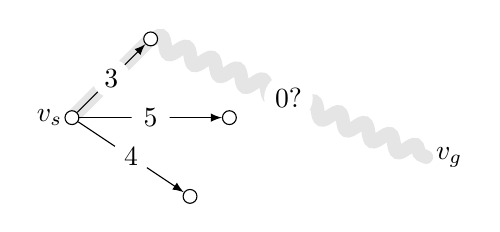
\begin{tikzpicture}
\tikzstyle{vertex}=[circle,draw=black,fill=white,inner sep=0pt,minimum size=5pt]

\coordinate (a) at (0,0);
\coordinate (b) at (2,0);
\coordinate (c) at (2.5,1);
\coordinate (d) at (1,1);
\coordinate (e) at (3,-0.5);
\coordinate (f) at (4,0.5);
\coordinate (g) at (4.5,-0.5);
\coordinate (h) at (1.5,-1);

\draw[black!10,line width=5pt,line cap=round] (a) -- (d);
\draw[black!10,line width=5pt,line cap=round,
   decorate,decoration=snake]
   (d) -- (g) node [black,circle,inner sep=2pt,midway,fill=white] {0?};

\node[vertex] (na) at (a) {};
\node[vertex] (nb) at (b) {};
%\node[vertex] (nc) at (c) {};
\node[vertex] (nd) at (d) {};
%\node[vertex] (ne) at (e) {};
%\node[vertex] (nf) at (f) {};
%\node[vertex] (ng) at (g) {};
\node[vertex] (nh) at (h) {};

\draw[black,->,>=latex] (na) -- (nb) node [circle,inner sep=2pt,midway,fill=white] {5};
\draw[black,->,>=latex] (na) -- (nh) node [circle,inner sep=2pt,midway,fill=white] {4};
\draw[black,->,>=latex] (na) -- (nd) node [circle,inner sep=2pt,midway,fill=white] {3};

\node[left=0pt of a] {$v_s$};
\node[right=0pt of g] {$v_g$};

\end{tikzpicture}
\caption{Select optimistic best path}
\end{subfigure}%
\quad%
\begin{subfigure}[b]{0.45\textwidth}
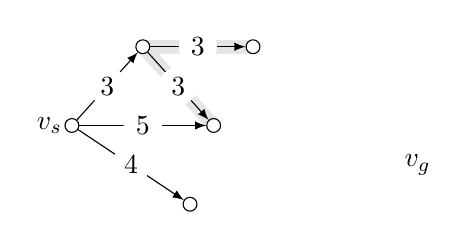
\begin{tikzpicture}
\tikzstyle{vertex}=[circle,draw=black,fill=white,inner sep=0pt,minimum size=5pt]

\coordinate (a) at (0,0);
\coordinate (b) at (1.8,0);
\coordinate (c) at (2.3,1);
\coordinate (d) at (0.9,1);
\coordinate (e) at (2.7,-0.5);
\coordinate (f) at (3.6,0.5);
\coordinate (g) at (4.1,-0.5);
\coordinate (h) at (1.5,-1);

\draw[black!10,line width=5pt,line cap=round] (d) -- (c);
\draw[black!10,line width=5pt,line cap=round] (d) -- (b);

\node[vertex] (na) at (a) {};
\node[vertex] (nb) at (b) {};
\node[vertex] (nc) at (c) {};
\node[vertex] (nd) at (d) {};
%\node[vertex] (ne) at (e) {};
%\node[vertex] (nf) at (f) {};
%\node[vertex] (ng) at (g) {};
\node[vertex] (nh) at (h) {};

\draw[black,->,>=latex] (na) -- (nb) node [circle,inner sep=2pt,midway,fill=white] {5};
\draw[black,->,>=latex] (na) -- (nh) node [circle,inner sep=2pt,midway,fill=white] {4};
\draw[black,->,>=latex] (na) -- (nd) node [circle,inner sep=2pt,midway,fill=white] {3};
\draw[black,->,>=latex] (nd) -- (nb) node [circle,inner sep=2pt,midway,fill=white] {3};
\draw[black,->,>=latex] (nd) -- (nc) node [circle,inner sep=2pt,midway,fill=white] {3};

\node[left=0pt of a] {$v_s$};
\node[right=0pt of g] {$v_g$};

\end{tikzpicture}
\caption{Expand first unexpanded vertex}
\end{subfigure}%
\caption{Best-first algorithm for an implicit graph,
   with $f(\pi)$ best known cost-from-start,
   and {\sc Eval} forward vertex expansions.
   This is Dijkstra's algorithm \cite{dijkstra1959anote}.}
\label{fig:seg-implicit}
\end{figure}

Takeaway: A* uses a general heuristic function $h_g(v)$
because it doesn't have a representation of the full graph,
so it can't compute an actual best optimistic path.
I claim that for manipulation planning problems,
we can indeed reason over explicit graphs.

\subsubsection{Relation to BHFFA}

Let's say that we also have a function which computes the predecessors
of a vertex,
and also an admissible heuristic function $h(v_a,v_b)$ which computes
a lower-bound estimate of the optimal cost between two vertices.
Then the best-first thing to do is equivalent to the
Bidirectional Heuristic Front-to-Front Algorithm \cite{sint1977bhffa}.

\subsection{Best-First Search with Edge Evaluation}

What if, instead of operating over vertices (like A* and the like),
we operate over edges?
Figure~\ref{fig:seg-intro} illustrated the simplest such algorithm,
which selects the optimistic-optimal path,
and then evaluates the first as-yet unevaluated edge on the path.

I think that the forward-evaluation version of this is the same as
Optimal Generation A* (OPA*) and Simple Optimal Generation A* (SOGA*)
\cite{goldenberg2013epeastar},
which are modified versions of
Enhanced Partial Expansion A* \cite{felner2012epastar}.

\subsection{Bidirectional {\sc Eval} Procedures}

In general, over explicit graphs,
it usually makes sense to do bidirectional evaluations.
I need some data to back this up for my problem.
For example,
the Lazy PRM algorithm \cite{bohlin2000lazyprm}
is just best-first search
applied to binary edge cost functions
($c(e) \in \{ \hat{c}(e), \infty \}$)
with bidirectional edge evaluations
(although it actually uses a slightly fancier path evaluation function).

\section{Penalizing Planning Effort}

So far, we've been searching for a path which optimizes our solution
cost objective (\ref{eqn:execution-cost-objective}).
However, as we motivated in the introduction,
there are two distint notions of efficency,
and our objective so far (\ref{eqn:execution-cost-objective})
has only captured one of the two.
Here, we focus instead on \emph{planning efficiency},
and attempt to define an objective which captures it.
We hope that doing so will lead to searches which consume less 
time or energy.

\begin{equation}
   f_p(\pi) = \mbox{\emph{optimistic estimate of planning effort}}.
\end{equation}

What type of metric should we use?

\subsection{Metrics for Planning Effort}

For problems over very large graphs,
planning effort may be dominated by expanding vertices
or maintaining priority queues.
Therefore, traditional metrics for evaluating planning
effort are \emph{vertices expanded}
and \emph{heap percolates}.
However, for many manipulation problems,
search time is instead dominated by edge evaluations.

Therefore, we introduce a new objective $f_p$
which penalizes effort spent evaluating edges along a potential path:
\begin{equation}
   f_p(\pi) = \sum_{e \in \pi} \left\{
   \begin{array}{cl}
      0 & \mbox{if edge } e \mbox{ evaluated}  \\
      \hat{p}(e) & \mbox{otherwise} \\
   \end{array}
   \right.
   .
\end{equation}
This uses a new heuristic $\hat{p}(e)$ which estimates the cost
associated with evaluating an edge.
This could be planning time, computational energy required, etc.

The first graph planner to explicitly include such a heuristic
to estimate the remaining
computational planning effort in a best-first search
was A$_\epsilon^*$ \cite{pearl1982semiadmissible}.
While the approach we take is different from that of
\cite{pearl1982semiadmissible},
a motivating quote from this paper is relevant:
\begin{quote}
``The heuristic [\,$\hat{c}$\,] ... is of an entirely
different nature than the ... heuristic [\,$\hat{p}$\,] ... .
The former anticipates the reduction in \emph{solution quality} due to the
remaining part of the solution once it is found;
the latter estimates the \emph{computational effort}
required for completing the search.''
\end{quote}

Sidenote: RRT-Connect is sort of explicitly doing this
(optimizing at each step only for planning time,
but constrained to pass through the sampled point).

\subsection{General Weighted Objective}

In general, we might consider weighting each objective:
\begin{equation}
   f(\pi) = \lambda f_p(\pi) + (1 - \lambda) f_x(\pi) .
   \label{eqn:general-objective}
\end{equation}
Note that with $\lambda=0$,
we recover our old solution cost objective $f_x(\pi)$.
Note that this objective is used in an optimistic, greedy fashion at each
iteration of best-first search.

This is the objective used by the Greedy PRM,
described in Section~\ref{sec:greedy-prm}.

When expanded,
this can then be written:
\begin{equation}
   f(\pi) = \sum_{e \in \pi} \left\{
   \begin{array}{cl}
      (1 - \lambda) c[e] & \mbox{if edge } e \mbox{ evaluated}  \\
      \lambda \hat{p}(e) + (1 - \lambda) \hat{c}(e) & \mbox{otherwise} \\
   \end{array}
   \right.
   .
   \label{eqn:general-objective-explicit}
\end{equation}

\subsection{Simplification with Propotional Heuristics}

Suppose that our edge evaluation cost heuristic
were proportional to our edge execution cost heuristic,
\begin{equation}
   \hat{p}(e) = \alpha \, \hat{c}(e) .
\end{equation}
This might happen if, for example, each were proportional to the edge's
\emph{distance} (with longer paths taking longer to both collision check
and execute at constant velocity).
In this case, we can write:
\begin{equation}
   f(\pi) = (1-\lambda) \sum_{e \in \pi} \left\{
   \begin{array}{cl}
      c[e] & \mbox{if edge } e \mbox{ evaluated}  \\
      \left[ 1 + \frac{\alpha\lambda}{1 - \lambda} \right] \hat{c}(e) & \mbox{otherwise} \\
   \end{array}
   \right.
   .
   \label{eqn:prop-heuristics}
\end{equation}

\subsection{Equivalence to Weighted A*}

Consider the case where we're using forward vertex or edge evaluations
(as is required with implicit graph representations),
and $\lambda < 1$.
In this case, we can rewrite (\ref{eqn:prop-heuristics})
simply as:
\begin{equation}
   f(\pi) \propto
   \underbrace{\sum_{e \; \mbox{\scriptsize evaled}} c[e]}_{g[v_f]}
   +
   \underbrace{\left[ 1 + \frac{\alpha \lambda}{1-\lambda} \right]}_{
      \mbox{\scriptsize inflation factor } \epsilon}
   \underbrace{\hat{c}(e_{last})}_{h(v_f)}
   .
\end{equation}

In other words,
\emph{weighted A* is simply best-first search whose objective
   includes a planning effort term.}

In particular, if planning effort is proportional to execution
effort by a factor of $\alpha$,
a weighted A* search with inflation factor $\epsilon$
is the result of best-first search with
$\lambda = \frac{\epsilon-1}{\alpha+\epsilon-1}$.

\subsection{Relation to Experience Graphs}
\label{sec:egraphs}

Experience graphs \cite{phillips2012egraphs}
are a type of best-first search which
are designed to find paths quickly by incentivizing the planner
to rely on on edges from previous successful plans.

While the E-graph planner is originally expressed over implicit graphs,
we can instead express it as best-first search over paths
with the following objective:
\begin{equation}
   f_{\mbox{\scriptsize E-graphs}}(\pi) \propto \sum_{e \in \pi} \left\{
   \begin{array}{cl}
      c[e] & \mbox{if edge } e \mbox{ evaluated, this search} \\
      \epsilon \, c[e] & \mbox{if edge } e \mbox{ evaluated, previous search} \\
     \epsilon \, \epsilon^E \, \hat{c}(e) & \mbox{otherwise} \\
   \end{array}
   \right.
   \label{eqn:prop-heuristics}
\end{equation}

The Greedy PRM applied to a single $C_{free}$ as described in this chapter
is equivalent to the E-Graph planner
with $\epsilon=1$ and $\epsilon^E = 1 + \frac{\alpha \lambda}{1-\lambda}$.
It's not immediately clear to me why one would choose $\epsilon \neq 1$.
(Note: we don't do shortcuts or snap motions.)

\section{Planner: Greedy PRM}
\label{sec:greedy-prm}

The Greedy PRM is the result of applying
best-first search with the $\lambda$-mediated objective
(\ref{eqn:general-objective})
to a simple single-$C_{free}$ problem
in batches of $N$ samples.
Based on empirical results, we also use the bidirectional edge evaluation
algorithn,
since it tends to finish faster.

\subsection{Implementation Details}

Talk about how the algorithm actually functions
(including all the speedups currently implemented,
plus new ones based on LPA* etc).

\subsection{Choosing $\lambda$}

Minimizing total time in a greedy fashion implies $\lambda = 0.5$.
For later steps in a multi-step plan,
we might have an estimate of the probability $P_e$ that the given query will
actually be executed.
We can then pose our optimistic objective as total planning and execution
time in expection;
this induces the following parameter choice:
\begin{equation}
   \lambda = \frac{1}{1 + P_e} .
\end{equation}
For example, $P_e=1$ induces $\lambda = 0.5$;
as $P_e \rightarrow 0$, $\lambda \rightarrow 1$.
In other words,
as the estimated probability of executing the path goes down,
the planner becomes greedier w.r.t. planning effort at the expense of
costlier solution paths.

This is all one-step greedy;
it returns the optimal path optimistically,
assuming it will be collision-free.
If we have some estimate of the proportion $P_u$ of evaluated edges
which will be part of the final path,
we can then choose a cost function which downweights the planning time.
I need to work this out. 

\subsection{Choosing Batch Size $N$}

What graph are we searching over?
If it's too sparse, we'll stop after knowing that no solution exists.
If it's too dense, we'll spend too much time filling in parts of
space.
There's actually some spatial relationship in $C_{free}$ what we're not
modeling.
We get around this with artificial sparseness.
There's definitely a paper's worth of work here too (Shushman's stuff).
The easy version is with sequential batches of size $N$.

Talk about how this is complementary to BIT* which acheive speedups
by batching, not by inflating.

\section{Results}

Here are results.
See Figure~\ref{fig:bean} and Figure~\ref{fig:herb-comparison-cdfs}.

I hope to show that the Greedy PRM is competitive with RRT-Connect
in terms of planning effort required to find a feasible path.

\begin{figure}
\centering
\begin{subfigure}[b]{0.3\textwidth}
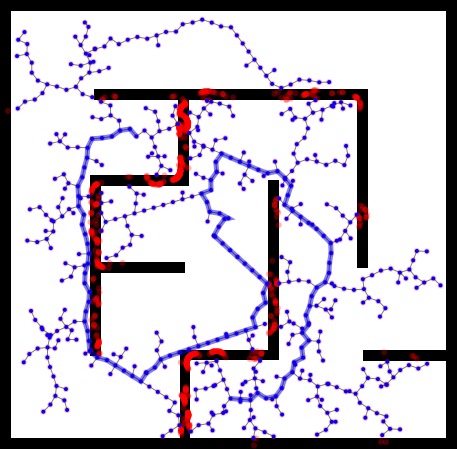
\includegraphics[width=\textwidth]{figs/compare-2d-rrtc1-rrtextcon-r1-s1.png}
\caption{RRT Ext-Con, R=1}
\end{subfigure}%
\quad
\begin{subfigure}[b]{0.3\textwidth}
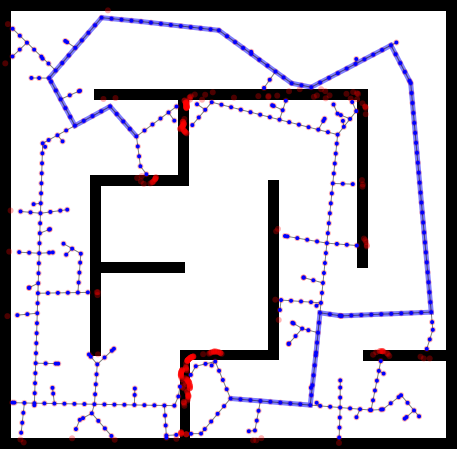
\includegraphics[width=\textwidth]{figs/compare-2d-rrtc1-rrtconcon-r1-s1.png}
\caption{RRT Con-Con, R=1}
\end{subfigure}%
\quad
\begin{subfigure}[b]{0.3\textwidth}
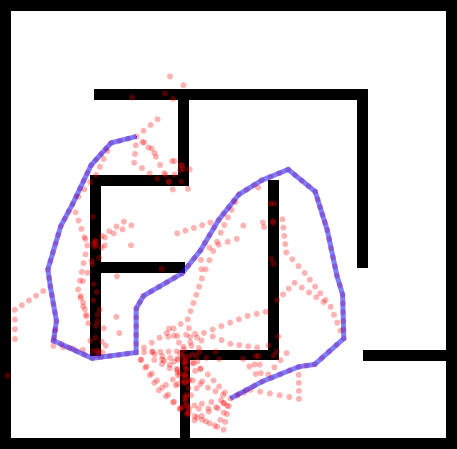
\includegraphics[width=\textwidth]{figs/compare-2d-rrtc1-checkmask-l00-s1.png}
\caption{Greedy PRM, $\lambda=0$}
\end{subfigure}%
\vspace{0.05in}
\begin{subfigure}[b]{0.3\textwidth}
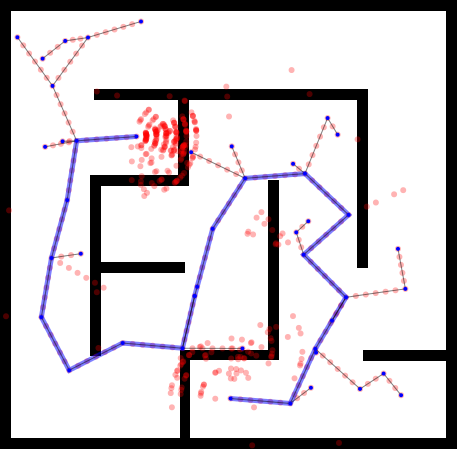
\includegraphics[width=\textwidth]{figs/compare-2d-rrtc1-rrtextcon-r6-s1.png}
\caption{RRT Ext-Con, R=6}
\end{subfigure}%
\quad
\begin{subfigure}[b]{0.3\textwidth}
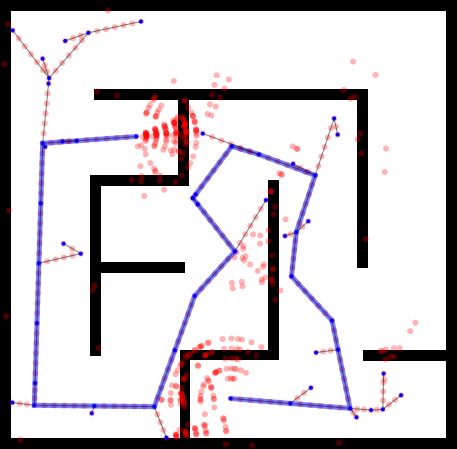
\includegraphics[width=\textwidth]{figs/compare-2d-rrtc1-rrtconcon-r6-s1.png}
\caption{RRT Con-Con, R=6}
\end{subfigure}%
\quad
\begin{subfigure}[b]{0.3\textwidth}
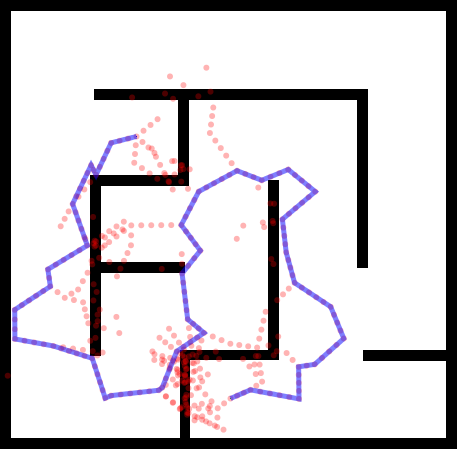
\includegraphics[width=\textwidth]{figs/compare-2d-rrtc1-checkmask-l10-s1.png}
\caption{Greedy PRM, $\lambda=1$}
\end{subfigure}%
\caption{Example runs with different planners,
   with the same sequence of samples.
   Note that Greedy PRM $\lambda=0$ is equivalent to LazyPRM.
   Red dots show collision checks.}
\label{fig:compare-2d-rrtc1-vis}
\end{figure}

\begin{figure}
\centering
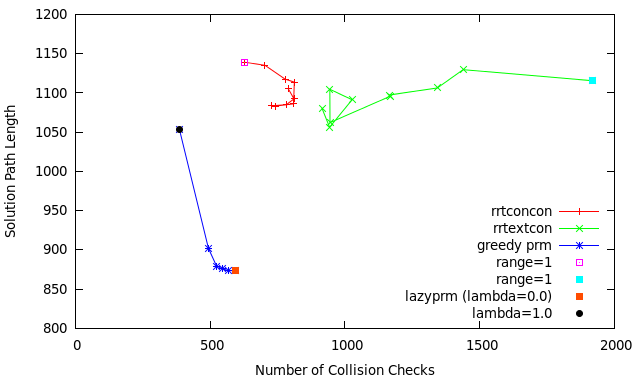
\includegraphics[width=0.8\textwidth]{figs/compare-2d-rrtc1-medians.png}
\caption{Plot of collision checks vs solution path cost for the
   different algorithms from the problem from
   Figure~\ref{fig:compare-2d-rrtc1-vis}.}
\end{figure}

\begin{figure}
\centering
\begin{subfigure}[b]{0.4\textwidth}
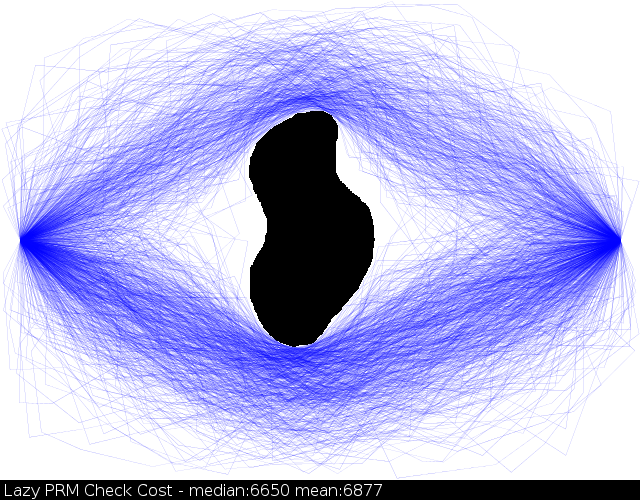
\includegraphics[width=\textwidth]{figs/timegreedy-bean-lambda-00.png}
\caption{Paths with $\lambda = 0$}
\end{subfigure}%
\quad
\begin{subfigure}[b]{0.4\textwidth}
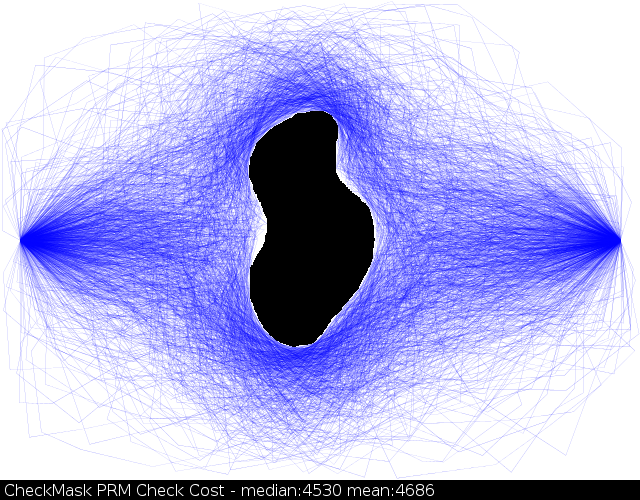
\includegraphics[width=\textwidth]{figs/timegreedy-bean-lambda-10.png}
\caption{Paths with $\lambda = 1$}
\end{subfigure}%
\caption{Examples of paths for a 2d problems
   for different values of $\lambda$.
   As $\lambda$ is increased,
   paths are longer, but are faster to find.}
\label{fig:bean}
\end{figure}

\begin{figure}
\centering
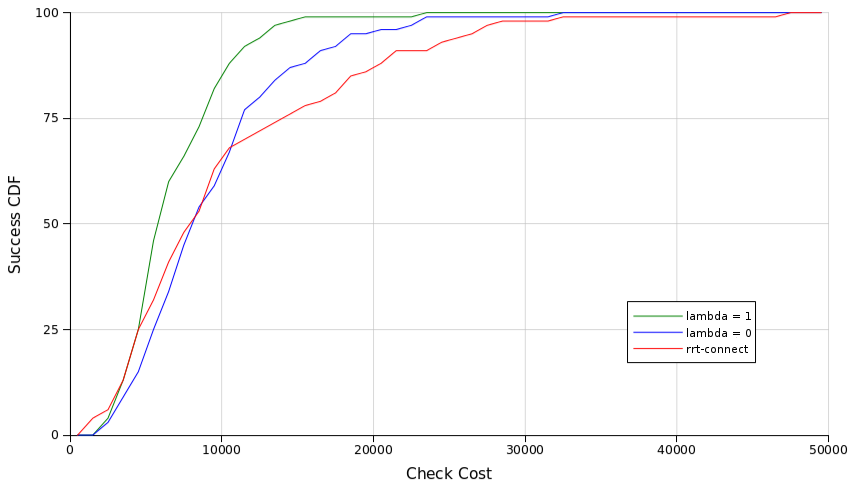
\includegraphics[width=0.8\textwidth]{figs/timegreedy-herbstep1-comparison-cdfs.png}
\caption{Comparison between different algorithms on a HERB problem.
   Must add in ESTs.}
\label{fig:herb-comparison-cdfs}
\end{figure}

\section{Repeated Queries}

For multiple queries within the same $C_{free}$,
the edge evaluations can be used in subsequent searches.
This ends up behaving similarily to E-graphs \cite{phillips2012egraphs}
with $\epsilon=1$
as described in Section~\ref{sec:egraphs},
with the exception that all evaluated edges are placed in the graph,
not just the edges on the solution path.

\section{Constraints}
\label{sec:constraints}

Here I talk about constrained planning.

\section{Future Work}

How to handle the narrow passage problem?
Lots of literature on that, new sampling strategies, etc.
(Toggle PRM, for instance.)



\newpage
\chapter{The Multi-Space Planning Problem}
\label{chap:multispace}

The purpose of this chapter is to introduce the multi-space planning
problem,
talk about its structure in general,
and show how about how a bunch of different problems in manipulation
are instances of this type of problem.

In the introduction to this chapter,
I'll talk about how the multi-step planning problem decomposition
discussed in Chapter~\ref{chap:formulation}
consists of a bunch of different queries in different
$C_{free}$s, but that are related.

For example, say you're planning to move an object from an initial
location to a goal location,
and then move your manipulator back to the start pose.
You have a single grasp for the object,
and your manipulator has a single IK for the grasp (very simple problem).
There are three $C_{free}$s here;
a naive approach would plan separately in each.

\section{Motivation}

Imagine a simple ``pick and place'' manipulation planning scenario
in which an articulated robot in a novel cluttered environment
is tasked with moving a particular object from a start pose to a goal
pose in the scene.

\begin{figure}
\centering
\begin{subfigure}[b]{0.3\textwidth}
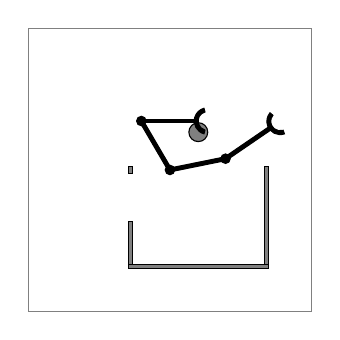
\begin{tikzpicture}
\begin{scope}[scale=1.2]
% bounding rect
\draw[color=black!50, thin] (-1.5,-1.5) rectangle (1.5,1.5);
\tikzstyle{dstyle}=[draw=black,fill=black!50]
\draw[dstyle] (0.300000,0.400000) circle (0.100000);
\draw[dstyle, shift={(0.300000,-1.020000)}, rotate=0.000000] (-0.740000,-0.020000) rectangle (0.740000,0.020000);
\draw[dstyle, shift={(1.020000,-0.480000)}, rotate=0.000000] (-0.020000,-0.520000) rectangle (0.020000,0.520000);
\draw[dstyle, shift={(-0.420000,-0.775000)}, rotate=0.000000] (-0.020000,-0.225000) rectangle (0.020000,0.225000);
\draw[dstyle, shift={(-0.420000,0.000000)}, rotate=0.000000] (-0.020000,-0.040000) rectangle (0.020000,0.040000);

\tikzstyle{dstyle}=[draw=black,fill=black]
\draw[dstyle] (0.000000,0.000000) circle (0.050000);
\draw[dstyle, shift={(0.294020,0.059601)}, rotate=11.459156] (-0.300000,-0.020000) rectangle (0.300000,0.020000);
\draw[dstyle] (0.588040,0.119202) circle (0.050000);
\draw[dstyle, shift={(1.165775,0.514451)}, rotate=214.377468](-74.484513:0.100000) arc (-74.484513:74.484513:0.100000) --(74.484513:0.140000) arc (74.484513:-74.484513:0.140000) -- cycle;
\draw[dstyle, shift={(0.835641,0.288594)}, rotate=34.377468] (-0.300000,-0.020000) rectangle (0.300000,0.020000);

%\tikzstyle{dstyle}=[draw=black!50]
%\draw[dstyle] (0.000000,0.000000) circle (0.050000);
\draw[dstyle, shift={(-0.151454,0.258963)}, rotate=120.321137] (-0.300000,-0.020000) rectangle (0.300000,0.020000);
\draw[dstyle] (-0.302908,0.517926) circle (0.050000);
\draw[dstyle, shift={(0.397092,0.517926)}, rotate=180.000000](-74.484513:0.100000) arc (-74.484513:74.484513:0.100000) --(74.484513:0.140000) arc (74.484513:-74.484513:0.140000) -- cycle;
\draw[dstyle, shift={(-0.002908,0.517926)}, rotate=0.000000] (-0.300000,-0.020000) rectangle (0.300000,0.020000);

\end{scope}
\end{tikzpicture}
\caption{Valid configuration}
\end{subfigure}%
\quad%
\begin{subfigure}[b]{0.3\textwidth}
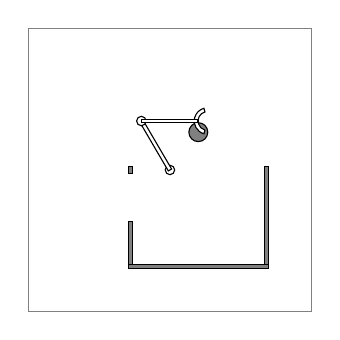
\begin{tikzpicture}
\begin{scope}[scale=1.2]
% bounding rect
\draw[color=black!50, thin] (-1.5,-1.5) rectangle (1.5,1.5);
\tikzstyle{dstyle}=[draw=black,fill=black!50]
\draw[dstyle] (0.300000,0.400000) circle (0.100000);
\draw[dstyle, shift={(0.300000,-1.020000)}, rotate=0.000000] (-0.740000,-0.020000) rectangle (0.740000,0.020000);
\draw[dstyle, shift={(1.020000,-0.480000)}, rotate=0.000000] (-0.020000,-0.520000) rectangle (0.020000,0.520000);
\draw[dstyle, shift={(-0.420000,-0.775000)}, rotate=0.000000] (-0.020000,-0.225000) rectangle (0.020000,0.225000);
\draw[dstyle, shift={(-0.420000,0.000000)}, rotate=0.000000] (-0.020000,-0.040000) rectangle (0.020000,0.040000);

\tikzstyle{dstyle}=[draw=black,fill=white]
\draw[dstyle] (0.000000,0.000000) circle (0.050000);
\draw[dstyle, shift={(-0.151454,0.258963)}, rotate=120.321137] (-0.300000,-0.020000) rectangle (0.300000,0.020000);
\draw[dstyle] (-0.302908,0.517926) circle (0.050000);
\draw[dstyle, shift={(0.397092,0.517926)}, rotate=180.000000](-74.484513:0.100000) arc (-74.484513:74.484513:0.100000) --(74.484513:0.140000) arc (74.484513:-74.484513:0.140000) -- cycle;
\draw[dstyle, shift={(-0.002908,0.517926)}, rotate=0.000000] (-0.300000,-0.020000) rectangle (0.300000,0.020000);

\end{scope}
\end{tikzpicture}
\caption{Invalid configuration}
\end{subfigure}%
\quad%
\begin{subfigure}[b]{0.3\textwidth}
\begin{tikzpicture}
\begin{scope}[scale=0.35]

\tikzstyle{every node}=[font=\scriptsize]

% x,y axes
\draw[->] (-3.14,-3.14) -- (4,-3.14) node[anchor=west] {$\theta_1$};
\draw[->] (-3.14,-3.14) -- (-3.14,4) node[anchor=south] {$\theta_2$};

% x tick marks with labels
\draw[-] (-3.14,-3.4) -- (-3.14,-3.14);
\draw[-] (    0,-3.4) -- (    0,-3.14);
\draw[-] ( 3.14,-3.4) -- ( 3.14,-3.14);
\draw	(-3.14,-3.4) node[anchor=north] {$-\pi$};
\draw	(    0,-3.4) node[anchor=north] {$0$};
\draw	( 3.14,-3.4) node[anchor=north] {$\pi$};

% y tick marks with labels
\draw[-] (-3.4,-3.14) -- (-3.14,-3.14);
\draw[-] (-3.4,    0) -- (-3.14,    0);
\draw[-] (-3.4, 3.14) -- (-3.14, 3.14);
\draw	(-3.4,-3.14) node[anchor=east] {$-\pi$};
\draw	(-3.4,    0) node[anchor=east] {$0$};
\draw	(-3.4, 3.14) node[anchor=east] {$\pi$};

% points
\draw[-,style=dotted] (0.2,-3.14) -- (0.2,0.4) -- (-3.14,0.4);
\draw[fill=black] (0.2,0.4) circle (0.15);
\draw[-,style=dotted] (2.1,-3.14) -- (2.1,-2.1) -- (-3.14,-2.1);
\draw[draw=black,fill=white] (2.1,-2.1) circle (0.15);

% legend
\draw[fill=black] (1,3.2) circle (0.15);
\draw	(1,3.2) node[anchor=west] {valid};
\draw[draw=black,fill=white] (1,2.3) circle (0.15);
\draw	(1,2.3) node[anchor=west] {invalid};

\end{scope}
\end{tikzpicture}
\caption{Configuration space}
\end{subfigure}
\caption{A simple planar 2-link manipulator problem.}
\end{figure}


\begin{figure}
\centering
\begin{subfigure}[b]{0.3\textwidth}
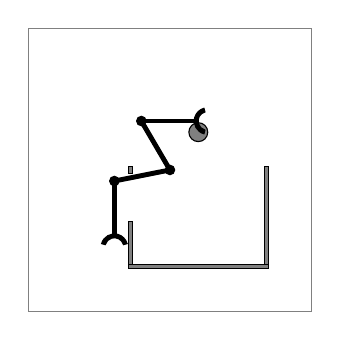
\begin{tikzpicture}
\begin{scope}[scale=1.2]
% bounding rect
\draw[color=black!50, thin] (-1.5,-1.5) rectangle (1.5,1.5);
\tikzstyle{dstyle}=[draw=black,fill=black!50]
\draw[dstyle] (0.300000,0.400000) circle (0.100000);
\draw[dstyle, shift={(0.300000,-1.020000)}, rotate=0.000000] (-0.740000,-0.020000) rectangle (0.740000,0.020000);
\draw[dstyle, shift={(1.020000,-0.480000)}, rotate=0.000000] (-0.020000,-0.520000) rectangle (0.020000,0.520000);
\draw[dstyle, shift={(-0.420000,-0.775000)}, rotate=0.000000] (-0.020000,-0.225000) rectangle (0.020000,0.225000);
\draw[dstyle, shift={(-0.420000,0.000000)}, rotate=0.000000] (-0.020000,-0.040000) rectangle (0.020000,0.040000);

\tikzstyle{dstyle}=[draw=black,fill=black]
\draw[dstyle] (0.000000,0.000000) circle (0.050000);
\draw[dstyle, shift={(-0.294233,-0.058540)}, rotate=-168.747530] (-0.300000,-0.020000) rectangle (0.300000,0.020000);
\draw[dstyle] (-0.588466,-0.117080) circle (0.050000);
\draw[dstyle, shift={(-0.588469,-0.817080)}, rotate=89.999790](-74.484513:0.100000) arc (-74.484513:74.484513:0.100000) --(74.484513:0.140000) arc (74.484513:-74.484513:0.140000) -- cycle;
\draw[dstyle, shift={(-0.588467,-0.417080)}, rotate=-90.000210] (-0.300000,-0.020000) rectangle (0.300000,0.020000);

%\tikzstyle{dstyle}=[draw=black!50]
%\draw[dstyle] (0.000000,0.000000) circle (0.050000);
\draw[dstyle, shift={(-0.151454,0.258963)}, rotate=120.321137] (-0.300000,-0.020000) rectangle (0.300000,0.020000);
\draw[dstyle] (-0.302908,0.517926) circle (0.050000);
\draw[dstyle, shift={(0.397092,0.517926)}, rotate=180.000000](-74.484513:0.100000) arc (-74.484513:74.484513:0.100000) --(74.484513:0.140000) arc (74.484513:-74.484513:0.140000) -- cycle;
\draw[dstyle, shift={(-0.002908,0.517926)}, rotate=0.000000] (-0.300000,-0.020000) rectangle (0.300000,0.020000);

\end{scope}
\end{tikzpicture}
\caption{Valid configuration}
\end{subfigure}%
\quad%
\begin{subfigure}[b]{0.3\textwidth}
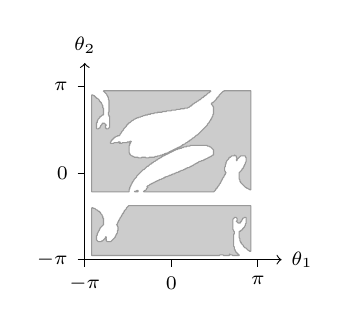
\begin{tikzpicture}
\begin{scope}[scale=0.35]

\tikzstyle{every node}=[font=\scriptsize]

% x,y axes
\draw[->] (-3.14,-3.14) -- (4,-3.14) node[anchor=west] {$\theta_1$};
\draw[->] (-3.14,-3.14) -- (-3.14,4) node[anchor=south] {$\theta_2$};

% x tick marks with labels
\draw[-] (-3.14,-3.4) -- (-3.14,-3.14);
\draw[-] (    0,-3.4) -- (    0,-3.14);
\draw[-] ( 3.14,-3.4) -- ( 3.14,-3.14);
\draw	(-3.14,-3.4) node[anchor=north] {$-\pi$};
\draw	(    0,-3.4) node[anchor=north] {$0$};
\draw	( 3.14,-3.4) node[anchor=north] {$\pi$};

% y tick marks with labels
\draw[-] (-3.4,-3.14) -- (-3.14,-3.14);
\draw[-] (-3.4,    0) -- (-3.14,    0);
\draw[-] (-3.4, 3.14) -- (-3.14, 3.14);
\draw	(-3.4,-3.14) node[anchor=east] {$-\pi$};
\draw	(-3.4,    0) node[anchor=east] {$0$};
\draw	(-3.4, 3.14) node[anchor=east] {$\pi$};

\begin{scope}[shift={(-3.14,-3.14)},scale=6.28]
\tikzstyle{fdstyle}=[color=black!40, fill=black!20, thin]
\filldraw[fdstyle, even odd rule]
   (0.254000,0.312000) -- (0.258000,0.312000) -- (0.262000,0.312000) -- (0.266000,0.312000) -- (0.270000,0.312000) -- (0.274000,0.312000) -- (0.278000,0.312000) -- (0.282000,0.312000) -- (0.286000,0.312000) -- (0.290000,0.312000) -- (0.294000,0.312000) -- (0.298000,0.312000) -- (0.302000,0.312000) -- (0.306000,0.312000) -- (0.310000,0.312000) -- (0.314000,0.312000) -- (0.318000,0.312000) -- (0.322000,0.312000) -- (0.326000,0.312000) -- (0.330000,0.312000) -- (0.334000,0.312000) -- (0.338000,0.312000) -- (0.342000,0.312000) -- (0.346000,0.312000) -- (0.350000,0.312000) -- (0.354000,0.312000) -- (0.358000,0.312000) -- (0.362000,0.312000) -- (0.366000,0.312000) -- (0.370000,0.312000) -- (0.374000,0.312000) -- (0.378000,0.312000) -- (0.382000,0.312000) -- (0.386000,0.312000) -- (0.390000,0.312000) -- (0.394000,0.312000) -- (0.398000,0.312000) -- (0.402000,0.312000) -- (0.406000,0.312000) -- (0.410000,0.312000) -- (0.414000,0.312000) -- (0.418000,0.312000) -- (0.422000,0.312000) -- (0.426000,0.312000) -- (0.430000,0.312000) -- (0.434000,0.312000) -- (0.438000,0.312000) -- (0.442000,0.312000) -- (0.446000,0.312000) -- (0.450000,0.312000) -- (0.454000,0.312000) -- (0.458000,0.312000) -- (0.462000,0.312000) -- (0.466000,0.312000) -- (0.470000,0.312000) -- (0.474000,0.312000) -- (0.478000,0.312000) -- (0.482000,0.312000) -- (0.486000,0.312000) -- (0.490000,0.312000) -- (0.494000,0.312000) -- (0.498000,0.312000) -- (0.502000,0.312000) -- (0.506000,0.312000) -- (0.510000,0.312000) -- (0.514000,0.312000) -- (0.518000,0.312000) -- (0.522000,0.312000) -- (0.526000,0.312000) -- (0.530000,0.312000) -- (0.534000,0.312000) -- (0.538000,0.312000) -- (0.542000,0.312000) -- (0.546000,0.312000) -- (0.550000,0.312000) -- (0.554000,0.312000) -- (0.558000,0.312000) -- (0.562000,0.312000) -- (0.566000,0.312000) -- (0.570000,0.312000) -- (0.574000,0.312000) -- (0.578000,0.312000) -- (0.582000,0.312000) -- (0.586000,0.312000) -- (0.590000,0.312000) -- (0.594000,0.312000) -- (0.598000,0.312000) -- (0.602000,0.312000) -- (0.606000,0.312000) -- (0.610000,0.312000) -- (0.614000,0.312000) -- (0.618000,0.312000) -- (0.622000,0.312000) -- (0.626000,0.312000) -- (0.630000,0.312000) -- (0.634000,0.312000) -- (0.638000,0.312000) -- (0.642000,0.312000) -- (0.646000,0.312000) -- (0.650000,0.312000) -- (0.654000,0.312000) -- (0.658000,0.312000) -- (0.662000,0.312000) -- (0.666000,0.312000) -- (0.670000,0.312000) -- (0.674000,0.312000) -- (0.678000,0.312000) -- (0.682000,0.312000) -- (0.686000,0.312000) -- (0.690000,0.312000) -- (0.694000,0.312000) -- (0.698000,0.312000) -- (0.702000,0.312000) -- (0.706000,0.312000) -- (0.710000,0.312000) -- (0.714000,0.312000) -- (0.718000,0.312000) -- (0.722000,0.312000) -- (0.726000,0.312000) -- (0.730000,0.312000) -- (0.734000,0.312000) -- (0.738000,0.312000) -- (0.742000,0.312000) -- (0.746000,0.312000) -- (0.750000,0.312000) -- (0.754000,0.312000) -- (0.758000,0.312000) -- (0.762000,0.312000) -- (0.766000,0.312000) -- (0.770000,0.312000) -- (0.774000,0.312000) -- (0.778000,0.312000) -- (0.782000,0.312000) -- (0.786000,0.312000) -- (0.790000,0.312000) -- (0.794000,0.312000) -- (0.798000,0.312000) -- (0.802000,0.312000) -- (0.806000,0.312000) -- (0.810000,0.312000) -- (0.814000,0.312000) -- (0.818000,0.312000) -- (0.822000,0.312000) -- (0.826000,0.312000) -- (0.830000,0.312000) -- (0.834000,0.312000) -- (0.838000,0.312000) -- (0.842000,0.312000) -- (0.846000,0.312000) -- (0.850000,0.312000) -- (0.854000,0.312000) -- (0.858000,0.312000) -- (0.862000,0.312000) -- (0.866000,0.312000) -- (0.870000,0.312000) -- (0.874000,0.312000) -- (0.878000,0.312000) -- (0.882000,0.312000) -- (0.886000,0.312000) -- (0.890000,0.312000) -- (0.894000,0.312000) -- (0.898000,0.312000) -- (0.902000,0.312000) -- (0.906000,0.312000) -- (0.910000,0.312000) -- (0.914000,0.312000) -- (0.918000,0.312000) -- (0.922000,0.312000) -- (0.926000,0.312000) -- (0.930000,0.312000) -- (0.934000,0.312000) -- (0.938000,0.312000) -- (0.942000,0.312000) -- (0.946000,0.312000) -- (0.950000,0.312000) -- (0.954000,0.312000) -- (0.958000,0.312000) -- (0.960000,0.310000) -- (0.960000,0.306000) -- (0.960000,0.302000) -- (0.960000,0.298000) -- (0.960000,0.294000) -- (0.960000,0.290000) -- (0.960000,0.286000) -- (0.960000,0.282000) -- (0.960000,0.278000) -- (0.960000,0.274000) -- (0.960000,0.270000) -- (0.960000,0.266000) -- (0.960000,0.262000) -- (0.960000,0.258000) -- (0.960000,0.254000) -- (0.960000,0.250000) -- (0.960000,0.246000) -- (0.960000,0.242000) -- (0.960000,0.238000) -- (0.960000,0.234000) -- (0.960000,0.230000) -- (0.960000,0.226000) -- (0.960000,0.222000) -- (0.960000,0.218000) -- (0.960000,0.214000) -- (0.960000,0.210000) -- (0.960000,0.206000) -- (0.960000,0.202000) -- (0.960000,0.198000) -- (0.960000,0.194000) -- (0.960000,0.190000) -- (0.960000,0.186000) -- (0.960000,0.182000) -- (0.960000,0.178000) -- (0.960000,0.174000) -- (0.960000,0.170000) -- (0.960000,0.166000) -- (0.960000,0.162000) -- (0.960000,0.158000) -- (0.960000,0.154000) -- (0.960000,0.150000) -- (0.960000,0.146000) -- (0.960000,0.142000) -- (0.960000,0.138000) -- (0.960000,0.134000) -- (0.960000,0.130000) -- (0.960000,0.126000) -- (0.960000,0.122000) -- (0.960000,0.118000) -- (0.960000,0.114000) -- (0.960000,0.110000) -- (0.960000,0.106000) -- (0.960000,0.102000) -- (0.960000,0.098000) -- (0.960000,0.094000) -- (0.960000,0.090000) -- (0.960000,0.086000) -- (0.960000,0.082000) -- (0.960000,0.078000) -- (0.960000,0.074000) -- (0.960000,0.070000) -- (0.960000,0.066000) -- (0.960000,0.062000) -- (0.960000,0.058000) -- (0.960000,0.054000) -- (0.960000,0.050000) -- (0.958000,0.048000) -- (0.954000,0.048000) -- (0.952000,0.050000) -- (0.950000,0.052000) -- (0.946000,0.052000) -- (0.944000,0.054000) -- (0.942000,0.056000) -- (0.940000,0.058000) -- (0.938000,0.060000) -- (0.936000,0.062000) -- (0.934000,0.064000) -- (0.932000,0.066000) -- (0.930000,0.068000) -- (0.926000,0.068000) -- (0.924000,0.070000) -- (0.922000,0.072000) -- (0.920000,0.074000) -- (0.918000,0.076000) -- (0.916000,0.078000) -- (0.916000,0.082000) -- (0.914000,0.084000) -- (0.912000,0.086000) -- (0.910000,0.088000) -- (0.908000,0.090000) -- (0.906000,0.092000) -- (0.904000,0.094000) -- (0.904000,0.098000) -- (0.902000,0.100000) -- (0.900000,0.102000) -- (0.900000,0.106000) -- (0.898000,0.108000) -- (0.896000,0.110000) -- (0.896000,0.114000) -- (0.896000,0.118000) -- (0.896000,0.122000) -- (0.894000,0.124000) -- (0.892000,0.126000) -- (0.892000,0.130000) -- (0.892000,0.134000) -- (0.892000,0.138000) -- (0.892000,0.142000) -- (0.892000,0.146000) -- (0.892000,0.150000) -- (0.892000,0.154000) -- (0.892000,0.158000) -- (0.892000,0.162000) -- (0.894000,0.164000) -- (0.898000,0.164000) -- (0.900000,0.166000) -- (0.902000,0.168000) -- (0.904000,0.170000) -- (0.906000,0.172000) -- (0.910000,0.172000) -- (0.912000,0.174000) -- (0.912000,0.178000) -- (0.914000,0.180000) -- (0.916000,0.182000) -- (0.918000,0.184000) -- (0.920000,0.186000) -- (0.922000,0.188000) -- (0.924000,0.190000) -- (0.924000,0.194000) -- (0.926000,0.196000) -- (0.928000,0.198000) -- (0.928000,0.202000) -- (0.928000,0.206000) -- (0.930000,0.208000) -- (0.932000,0.210000) -- (0.932000,0.214000) -- (0.932000,0.218000) -- (0.932000,0.222000) -- (0.932000,0.226000) -- (0.932000,0.230000) -- (0.932000,0.234000) -- (0.932000,0.238000) -- (0.932000,0.242000) -- (0.930000,0.244000) -- (0.926000,0.244000) -- (0.922000,0.244000) -- (0.920000,0.242000) -- (0.918000,0.240000) -- (0.914000,0.240000) -- (0.912000,0.238000) -- (0.912000,0.234000) -- (0.910000,0.232000) -- (0.908000,0.230000) -- (0.908000,0.226000) -- (0.906000,0.224000) -- (0.904000,0.222000) -- (0.902000,0.220000) -- (0.900000,0.218000) -- (0.900000,0.214000) -- (0.898000,0.212000) -- (0.894000,0.212000) -- (0.890000,0.212000) -- (0.886000,0.212000) -- (0.884000,0.214000) -- (0.882000,0.216000) -- (0.880000,0.218000) -- (0.878000,0.220000) -- (0.876000,0.222000) -- (0.878000,0.224000) -- (0.880000,0.226000) -- (0.880000,0.230000) -- (0.880000,0.234000) -- (0.880000,0.238000) -- (0.878000,0.240000) -- (0.876000,0.242000) -- (0.874000,0.244000) -- (0.870000,0.244000) -- (0.866000,0.244000) -- (0.864000,0.242000) -- (0.862000,0.240000) -- (0.860000,0.238000) -- (0.858000,0.236000) -- (0.856000,0.234000) -- (0.856000,0.230000) -- (0.856000,0.226000) -- (0.856000,0.222000) -- (0.856000,0.218000) -- (0.856000,0.214000) -- (0.856000,0.210000) -- (0.856000,0.206000) -- (0.856000,0.202000) -- (0.856000,0.198000) -- (0.856000,0.194000) -- (0.856000,0.190000) -- (0.856000,0.186000) -- (0.856000,0.182000) -- (0.856000,0.178000) -- (0.856000,0.174000) -- (0.858000,0.172000) -- (0.860000,0.170000) -- (0.860000,0.166000) -- (0.862000,0.164000) -- (0.864000,0.162000) -- (0.864000,0.158000) -- (0.864000,0.154000) -- (0.864000,0.150000) -- (0.862000,0.148000) -- (0.860000,0.146000) -- (0.860000,0.142000) -- (0.860000,0.138000) -- (0.860000,0.134000) -- (0.860000,0.130000) -- (0.860000,0.126000) -- (0.860000,0.122000) -- (0.860000,0.118000) -- (0.860000,0.114000) -- (0.860000,0.110000) -- (0.860000,0.106000) -- (0.860000,0.102000) -- (0.860000,0.098000) -- (0.860000,0.094000) -- (0.860000,0.090000) -- (0.860000,0.086000) -- (0.860000,0.082000) -- (0.860000,0.078000) -- (0.862000,0.076000) -- (0.864000,0.074000) -- (0.864000,0.070000) -- (0.864000,0.066000) -- (0.864000,0.062000) -- (0.866000,0.060000) -- (0.868000,0.058000) -- (0.868000,0.054000) -- (0.870000,0.052000) -- (0.872000,0.050000) -- (0.872000,0.046000) -- (0.874000,0.044000) -- (0.876000,0.042000) -- (0.878000,0.040000) -- (0.880000,0.038000) -- (0.882000,0.036000) -- (0.884000,0.034000) -- (0.886000,0.032000) -- (0.888000,0.030000) -- (0.890000,0.028000) -- (0.892000,0.026000) -- (0.890000,0.024000) -- (0.886000,0.024000) -- (0.882000,0.024000) -- (0.878000,0.024000) -- (0.874000,0.024000) -- (0.870000,0.024000) -- (0.866000,0.024000) -- (0.862000,0.024000) -- (0.858000,0.024000) -- (0.854000,0.024000) -- (0.852000,0.026000) -- (0.850000,0.028000) -- (0.846000,0.028000) -- (0.842000,0.028000) -- (0.840000,0.030000) -- (0.838000,0.032000) -- (0.836000,0.030000) -- (0.836000,0.026000) -- (0.834000,0.024000) -- (0.830000,0.024000) -- (0.826000,0.024000) -- (0.822000,0.024000) -- (0.818000,0.024000) -- (0.814000,0.024000) -- (0.810000,0.024000) -- (0.806000,0.024000) -- (0.802000,0.024000) -- (0.800000,0.026000) -- (0.798000,0.028000) -- (0.794000,0.028000) -- (0.790000,0.028000) -- (0.786000,0.028000) -- (0.782000,0.028000) -- (0.780000,0.026000) -- (0.778000,0.024000) -- (0.774000,0.024000) -- (0.770000,0.024000) -- (0.766000,0.024000) -- (0.762000,0.024000) -- (0.758000,0.024000) -- (0.754000,0.024000) -- (0.750000,0.024000) -- (0.746000,0.024000) -- (0.742000,0.024000) -- (0.738000,0.024000) -- (0.734000,0.024000) -- (0.730000,0.024000) -- (0.726000,0.024000) -- (0.722000,0.024000) -- (0.718000,0.024000) -- (0.714000,0.024000) -- (0.710000,0.024000) -- (0.706000,0.024000) -- (0.702000,0.024000) -- (0.698000,0.024000) -- (0.694000,0.024000) -- (0.690000,0.024000) -- (0.686000,0.024000) -- (0.682000,0.024000) -- (0.678000,0.024000) -- (0.674000,0.024000) -- (0.670000,0.024000) -- (0.666000,0.024000) -- (0.662000,0.024000) -- (0.658000,0.024000) -- (0.654000,0.024000) -- (0.650000,0.024000) -- (0.646000,0.024000) -- (0.642000,0.024000) -- (0.638000,0.024000) -- (0.634000,0.024000) -- (0.630000,0.024000) -- (0.626000,0.024000) -- (0.622000,0.024000) -- (0.618000,0.024000) -- (0.614000,0.024000) -- (0.610000,0.024000) -- (0.606000,0.024000) -- (0.602000,0.024000) -- (0.598000,0.024000) -- (0.594000,0.024000) -- (0.590000,0.024000) -- (0.586000,0.024000) -- (0.582000,0.024000) -- (0.578000,0.024000) -- (0.574000,0.024000) -- (0.570000,0.024000) -- (0.566000,0.024000) -- (0.562000,0.024000) -- (0.558000,0.024000) -- (0.554000,0.024000) -- (0.550000,0.024000) -- (0.546000,0.024000) -- (0.542000,0.024000) -- (0.538000,0.024000) -- (0.534000,0.024000) -- (0.530000,0.024000) -- (0.526000,0.024000) -- (0.522000,0.024000) -- (0.518000,0.024000) -- (0.514000,0.024000) -- (0.510000,0.024000) -- (0.506000,0.024000) -- (0.502000,0.024000) -- (0.498000,0.024000) -- (0.494000,0.024000) -- (0.490000,0.024000) -- (0.486000,0.024000) -- (0.482000,0.024000) -- (0.478000,0.024000) -- (0.474000,0.024000) -- (0.470000,0.024000) -- (0.466000,0.024000) -- (0.462000,0.024000) -- (0.458000,0.024000) -- (0.454000,0.024000) -- (0.450000,0.024000) -- (0.446000,0.024000) -- (0.442000,0.024000) -- (0.438000,0.024000) -- (0.434000,0.024000) -- (0.430000,0.024000) -- (0.426000,0.024000) -- (0.422000,0.024000) -- (0.418000,0.024000) -- (0.414000,0.024000) -- (0.410000,0.024000) -- (0.406000,0.024000) -- (0.402000,0.024000) -- (0.398000,0.024000) -- (0.394000,0.024000) -- (0.390000,0.024000) -- (0.386000,0.024000) -- (0.382000,0.024000) -- (0.378000,0.024000) -- (0.374000,0.024000) -- (0.370000,0.024000) -- (0.366000,0.024000) -- (0.362000,0.024000) -- (0.358000,0.024000) -- (0.354000,0.024000) -- (0.350000,0.024000) -- (0.346000,0.024000) -- (0.342000,0.024000) -- (0.338000,0.024000) -- (0.334000,0.024000) -- (0.330000,0.024000) -- (0.326000,0.024000) -- (0.322000,0.024000) -- (0.318000,0.024000) -- (0.314000,0.024000) -- (0.310000,0.024000) -- (0.306000,0.024000) -- (0.302000,0.024000) -- (0.298000,0.024000) -- (0.294000,0.024000) -- (0.290000,0.024000) -- (0.286000,0.024000) -- (0.282000,0.024000) -- (0.278000,0.024000) -- (0.274000,0.024000) -- (0.270000,0.024000) -- (0.266000,0.024000) -- (0.262000,0.024000) -- (0.258000,0.024000) -- (0.254000,0.024000) -- (0.250000,0.024000) -- (0.246000,0.024000) -- (0.242000,0.024000) -- (0.238000,0.024000) -- (0.234000,0.024000) -- (0.230000,0.024000) -- (0.226000,0.024000) -- (0.222000,0.024000) -- (0.218000,0.024000) -- (0.214000,0.024000) -- (0.210000,0.024000) -- (0.206000,0.024000) -- (0.202000,0.024000) -- (0.198000,0.024000) -- (0.194000,0.024000) -- (0.190000,0.024000) -- (0.186000,0.024000) -- (0.182000,0.024000) -- (0.178000,0.024000) -- (0.174000,0.024000) -- (0.170000,0.024000) -- (0.166000,0.024000) -- (0.162000,0.024000) -- (0.158000,0.024000) -- (0.154000,0.024000) -- (0.150000,0.024000) -- (0.146000,0.024000) -- (0.142000,0.024000) -- (0.138000,0.024000) -- (0.134000,0.024000) -- (0.130000,0.024000) -- (0.126000,0.024000) -- (0.122000,0.024000) -- (0.118000,0.024000) -- (0.114000,0.024000) -- (0.110000,0.024000) -- (0.106000,0.024000) -- (0.102000,0.024000) -- (0.098000,0.024000) -- (0.094000,0.024000) -- (0.090000,0.024000) -- (0.086000,0.024000) -- (0.082000,0.024000) -- (0.078000,0.024000) -- (0.074000,0.024000) -- (0.070000,0.024000) -- (0.066000,0.024000) -- (0.062000,0.024000) -- (0.058000,0.024000) -- (0.054000,0.024000) -- (0.050000,0.024000) -- (0.046000,0.024000) -- (0.042000,0.024000) -- (0.040000,0.026000) -- (0.040000,0.030000) -- (0.040000,0.034000) -- (0.040000,0.038000) -- (0.040000,0.042000) -- (0.040000,0.046000) -- (0.040000,0.050000) -- (0.040000,0.054000) -- (0.040000,0.058000) -- (0.040000,0.062000) -- (0.040000,0.066000) -- (0.040000,0.070000) -- (0.040000,0.074000) -- (0.040000,0.078000) -- (0.040000,0.082000) -- (0.040000,0.086000) -- (0.040000,0.090000) -- (0.040000,0.094000) -- (0.040000,0.098000) -- (0.040000,0.102000) -- (0.040000,0.106000) -- (0.040000,0.110000) -- (0.040000,0.114000) -- (0.040000,0.118000) -- (0.040000,0.122000) -- (0.040000,0.126000) -- (0.040000,0.130000) -- (0.040000,0.134000) -- (0.040000,0.138000) -- (0.040000,0.142000) -- (0.040000,0.146000) -- (0.040000,0.150000) -- (0.040000,0.154000) -- (0.040000,0.158000) -- (0.040000,0.162000) -- (0.040000,0.166000) -- (0.040000,0.170000) -- (0.040000,0.174000) -- (0.040000,0.178000) -- (0.040000,0.182000) -- (0.040000,0.186000) -- (0.040000,0.190000) -- (0.040000,0.194000) -- (0.040000,0.198000) -- (0.040000,0.202000) -- (0.040000,0.206000) -- (0.040000,0.210000) -- (0.040000,0.214000) -- (0.040000,0.218000) -- (0.040000,0.222000) -- (0.040000,0.226000) -- (0.040000,0.230000) -- (0.040000,0.234000) -- (0.040000,0.238000) -- (0.040000,0.242000) -- (0.040000,0.246000) -- (0.040000,0.250000) -- (0.040000,0.254000) -- (0.040000,0.258000) -- (0.040000,0.262000) -- (0.040000,0.266000) -- (0.040000,0.270000) -- (0.040000,0.274000) -- (0.040000,0.278000) -- (0.040000,0.282000) -- (0.040000,0.286000) -- (0.040000,0.290000) -- (0.040000,0.294000) -- (0.040000,0.298000) -- (0.042000,0.300000) -- (0.046000,0.300000) -- (0.048000,0.298000) -- (0.050000,0.296000) -- (0.054000,0.296000) -- (0.058000,0.296000) -- (0.060000,0.294000) -- (0.062000,0.292000) -- (0.064000,0.290000) -- (0.066000,0.288000) -- (0.070000,0.288000) -- (0.072000,0.286000) -- (0.074000,0.284000) -- (0.076000,0.282000) -- (0.078000,0.280000) -- (0.082000,0.280000) -- (0.084000,0.278000) -- (0.086000,0.276000) -- (0.088000,0.274000) -- (0.090000,0.272000) -- (0.092000,0.270000) -- (0.092000,0.266000) -- (0.094000,0.264000) -- (0.096000,0.262000) -- (0.098000,0.260000) -- (0.100000,0.258000) -- (0.100000,0.254000) -- (0.102000,0.252000) -- (0.104000,0.250000) -- (0.104000,0.246000) -- (0.104000,0.242000) -- (0.106000,0.240000) -- (0.108000,0.238000) -- (0.108000,0.234000) -- (0.108000,0.230000) -- (0.108000,0.226000) -- (0.108000,0.222000) -- (0.108000,0.218000) -- (0.108000,0.214000) -- (0.108000,0.210000) -- (0.108000,0.206000) -- (0.108000,0.202000) -- (0.106000,0.200000) -- (0.104000,0.198000) -- (0.102000,0.196000) -- (0.100000,0.194000) -- (0.098000,0.192000) -- (0.096000,0.190000) -- (0.094000,0.188000) -- (0.092000,0.186000) -- (0.090000,0.184000) -- (0.088000,0.182000) -- (0.088000,0.178000) -- (0.086000,0.176000) -- (0.084000,0.174000) -- (0.084000,0.170000) -- (0.082000,0.168000) -- (0.080000,0.166000) -- (0.080000,0.162000) -- (0.078000,0.160000) -- (0.076000,0.158000) -- (0.076000,0.154000) -- (0.074000,0.152000) -- (0.072000,0.150000) -- (0.072000,0.146000) -- (0.072000,0.142000) -- (0.070000,0.140000) -- (0.068000,0.138000) -- (0.068000,0.134000) -- (0.068000,0.130000) -- (0.068000,0.126000) -- (0.068000,0.122000) -- (0.068000,0.118000) -- (0.068000,0.114000) -- (0.070000,0.112000) -- (0.072000,0.110000) -- (0.074000,0.108000) -- (0.076000,0.106000) -- (0.078000,0.104000) -- (0.082000,0.104000) -- (0.086000,0.104000) -- (0.090000,0.104000) -- (0.094000,0.104000) -- (0.096000,0.106000) -- (0.098000,0.108000) -- (0.102000,0.108000) -- (0.104000,0.110000) -- (0.106000,0.112000) -- (0.108000,0.114000) -- (0.110000,0.116000) -- (0.112000,0.118000) -- (0.114000,0.120000) -- (0.116000,0.122000) -- (0.118000,0.124000) -- (0.120000,0.126000) -- (0.120000,0.130000) -- (0.122000,0.132000) -- (0.124000,0.130000) -- (0.124000,0.126000) -- (0.122000,0.124000) -- (0.120000,0.122000) -- (0.122000,0.120000) -- (0.124000,0.118000) -- (0.124000,0.114000) -- (0.124000,0.110000) -- (0.126000,0.108000) -- (0.128000,0.106000) -- (0.130000,0.104000) -- (0.134000,0.104000) -- (0.138000,0.104000) -- (0.142000,0.104000) -- (0.146000,0.104000) -- (0.150000,0.104000) -- (0.152000,0.106000) -- (0.154000,0.108000) -- (0.156000,0.110000) -- (0.158000,0.112000) -- (0.160000,0.114000) -- (0.162000,0.116000) -- (0.164000,0.118000) -- (0.166000,0.120000) -- (0.168000,0.122000) -- (0.170000,0.124000) -- (0.172000,0.126000) -- (0.174000,0.128000) -- (0.176000,0.130000) -- (0.176000,0.134000) -- (0.178000,0.136000) -- (0.180000,0.138000) -- (0.180000,0.142000) -- (0.182000,0.144000) -- (0.184000,0.146000) -- (0.184000,0.150000) -- (0.186000,0.152000) -- (0.188000,0.154000) -- (0.188000,0.158000) -- (0.188000,0.162000) -- (0.188000,0.166000) -- (0.190000,0.168000) -- (0.192000,0.170000) -- (0.192000,0.174000) -- (0.192000,0.178000) -- (0.192000,0.182000) -- (0.192000,0.186000) -- (0.192000,0.190000) -- (0.190000,0.192000) -- (0.188000,0.194000) -- (0.188000,0.198000) -- (0.186000,0.200000) -- (0.184000,0.202000) -- (0.186000,0.204000) -- (0.188000,0.206000) -- (0.188000,0.210000) -- (0.190000,0.212000) -- (0.192000,0.214000) -- (0.192000,0.218000) -- (0.194000,0.220000) -- (0.196000,0.222000) -- (0.196000,0.226000) -- (0.198000,0.228000) -- (0.200000,0.230000) -- (0.200000,0.234000) -- (0.202000,0.236000) -- (0.204000,0.238000) -- (0.204000,0.242000) -- (0.206000,0.244000) -- (0.208000,0.246000) -- (0.210000,0.248000) -- (0.212000,0.250000) -- (0.212000,0.254000) -- (0.214000,0.256000) -- (0.216000,0.258000) -- (0.216000,0.262000) -- (0.218000,0.264000) -- (0.220000,0.266000) -- (0.222000,0.268000) -- (0.224000,0.270000) -- (0.224000,0.274000) -- (0.226000,0.276000) -- (0.228000,0.278000) -- (0.228000,0.282000) -- (0.230000,0.284000) -- (0.232000,0.286000) -- (0.234000,0.288000) -- (0.236000,0.290000) -- (0.238000,0.292000) -- (0.240000,0.294000) -- (0.240000,0.298000) -- (0.242000,0.300000) -- (0.244000,0.302000) -- (0.246000,0.304000) -- (0.248000,0.306000) -- (0.250000,0.308000) -- (0.252000,0.310000) -- cycle
   (0.302000,0.400000) -- (0.306000,0.400000) -- (0.308000,0.398000) -- (0.308000,0.394000) -- (0.306000,0.392000) -- (0.302000,0.392000) -- (0.298000,0.392000) -- (0.294000,0.392000) -- (0.290000,0.392000) -- (0.288000,0.394000) -- (0.290000,0.396000) -- (0.294000,0.396000) -- (0.298000,0.396000) -- (0.300000,0.398000) -- cycle
   (0.110000,0.976000) -- (0.114000,0.976000) -- (0.118000,0.976000) -- (0.122000,0.976000) -- (0.126000,0.976000) -- (0.130000,0.976000) -- (0.134000,0.976000) -- (0.138000,0.976000) -- (0.142000,0.976000) -- (0.146000,0.976000) -- (0.150000,0.976000) -- (0.154000,0.976000) -- (0.158000,0.976000) -- (0.162000,0.976000) -- (0.166000,0.976000) -- (0.170000,0.976000) -- (0.174000,0.976000) -- (0.178000,0.976000) -- (0.182000,0.976000) -- (0.186000,0.976000) -- (0.190000,0.976000) -- (0.194000,0.976000) -- (0.198000,0.976000) -- (0.202000,0.976000) -- (0.206000,0.976000) -- (0.210000,0.976000) -- (0.214000,0.976000) -- (0.218000,0.976000) -- (0.222000,0.976000) -- (0.226000,0.976000) -- (0.230000,0.976000) -- (0.234000,0.976000) -- (0.238000,0.976000) -- (0.242000,0.976000) -- (0.246000,0.976000) -- (0.250000,0.976000) -- (0.254000,0.976000) -- (0.258000,0.976000) -- (0.262000,0.976000) -- (0.266000,0.976000) -- (0.270000,0.976000) -- (0.274000,0.976000) -- (0.278000,0.976000) -- (0.282000,0.976000) -- (0.286000,0.976000) -- (0.290000,0.976000) -- (0.294000,0.976000) -- (0.298000,0.976000) -- (0.302000,0.976000) -- (0.306000,0.976000) -- (0.310000,0.976000) -- (0.314000,0.976000) -- (0.318000,0.976000) -- (0.322000,0.976000) -- (0.326000,0.976000) -- (0.330000,0.976000) -- (0.334000,0.976000) -- (0.338000,0.976000) -- (0.342000,0.976000) -- (0.346000,0.976000) -- (0.350000,0.976000) -- (0.354000,0.976000) -- (0.358000,0.976000) -- (0.362000,0.976000) -- (0.366000,0.976000) -- (0.370000,0.976000) -- (0.374000,0.976000) -- (0.378000,0.976000) -- (0.382000,0.976000) -- (0.386000,0.976000) -- (0.390000,0.976000) -- (0.394000,0.976000) -- (0.398000,0.976000) -- (0.402000,0.976000) -- (0.406000,0.976000) -- (0.410000,0.976000) -- (0.414000,0.976000) -- (0.418000,0.976000) -- (0.422000,0.976000) -- (0.426000,0.976000) -- (0.430000,0.976000) -- (0.434000,0.976000) -- (0.438000,0.976000) -- (0.442000,0.976000) -- (0.446000,0.976000) -- (0.450000,0.976000) -- (0.454000,0.976000) -- (0.458000,0.976000) -- (0.462000,0.976000) -- (0.466000,0.976000) -- (0.470000,0.976000) -- (0.474000,0.976000) -- (0.478000,0.976000) -- (0.482000,0.976000) -- (0.486000,0.976000) -- (0.490000,0.976000) -- (0.494000,0.976000) -- (0.498000,0.976000) -- (0.502000,0.976000) -- (0.506000,0.976000) -- (0.510000,0.976000) -- (0.514000,0.976000) -- (0.518000,0.976000) -- (0.522000,0.976000) -- (0.526000,0.976000) -- (0.530000,0.976000) -- (0.534000,0.976000) -- (0.538000,0.976000) -- (0.542000,0.976000) -- (0.546000,0.976000) -- (0.550000,0.976000) -- (0.554000,0.976000) -- (0.558000,0.976000) -- (0.562000,0.976000) -- (0.566000,0.976000) -- (0.570000,0.976000) -- (0.574000,0.976000) -- (0.578000,0.976000) -- (0.582000,0.976000) -- (0.586000,0.976000) -- (0.590000,0.976000) -- (0.594000,0.976000) -- (0.598000,0.976000) -- (0.602000,0.976000) -- (0.606000,0.976000) -- (0.610000,0.976000) -- (0.614000,0.976000) -- (0.618000,0.976000) -- (0.622000,0.976000) -- (0.626000,0.976000) -- (0.630000,0.976000) -- (0.634000,0.976000) -- (0.638000,0.976000) -- (0.642000,0.976000) -- (0.646000,0.976000) -- (0.650000,0.976000) -- (0.654000,0.976000) -- (0.658000,0.976000) -- (0.662000,0.976000) -- (0.666000,0.976000) -- (0.670000,0.976000) -- (0.674000,0.976000) -- (0.678000,0.976000) -- (0.682000,0.976000) -- (0.686000,0.976000) -- (0.690000,0.976000) -- (0.694000,0.976000) -- (0.698000,0.976000) -- (0.702000,0.976000) -- (0.706000,0.976000) -- (0.710000,0.976000) -- (0.714000,0.976000) -- (0.718000,0.976000) -- (0.722000,0.976000) -- (0.726000,0.976000) -- (0.728000,0.974000) -- (0.726000,0.972000) -- (0.724000,0.970000) -- (0.722000,0.968000) -- (0.720000,0.966000) -- (0.718000,0.964000) -- (0.714000,0.964000) -- (0.712000,0.962000) -- (0.710000,0.960000) -- (0.708000,0.958000) -- (0.706000,0.956000) -- (0.704000,0.954000) -- (0.702000,0.952000) -- (0.700000,0.950000) -- (0.698000,0.948000) -- (0.694000,0.948000) -- (0.692000,0.946000) -- (0.690000,0.944000) -- (0.688000,0.942000) -- (0.686000,0.940000) -- (0.684000,0.938000) -- (0.682000,0.936000) -- (0.678000,0.936000) -- (0.676000,0.934000) -- (0.674000,0.932000) -- (0.672000,0.930000) -- (0.670000,0.928000) -- (0.668000,0.926000) -- (0.666000,0.924000) -- (0.662000,0.924000) -- (0.660000,0.922000) -- (0.658000,0.920000) -- (0.656000,0.918000) -- (0.654000,0.916000) -- (0.650000,0.916000) -- (0.648000,0.914000) -- (0.646000,0.912000) -- (0.644000,0.910000) -- (0.642000,0.908000) -- (0.638000,0.908000) -- (0.636000,0.906000) -- (0.634000,0.904000) -- (0.632000,0.902000) -- (0.630000,0.900000) -- (0.626000,0.900000) -- (0.624000,0.898000) -- (0.622000,0.896000) -- (0.620000,0.894000) -- (0.618000,0.892000) -- (0.616000,0.890000) -- (0.614000,0.888000) -- (0.610000,0.888000) -- (0.608000,0.886000) -- (0.606000,0.884000) -- (0.604000,0.882000) -- (0.602000,0.880000) -- (0.598000,0.880000) -- (0.596000,0.878000) -- (0.594000,0.876000) -- (0.590000,0.876000) -- (0.586000,0.876000) -- (0.582000,0.876000) -- (0.578000,0.876000) -- (0.576000,0.874000) -- (0.574000,0.872000) -- (0.570000,0.872000) -- (0.566000,0.872000) -- (0.562000,0.872000) -- (0.558000,0.872000) -- (0.554000,0.872000) -- (0.552000,0.870000) -- (0.550000,0.868000) -- (0.546000,0.868000) -- (0.542000,0.868000) -- (0.538000,0.868000) -- (0.534000,0.868000) -- (0.530000,0.868000) -- (0.528000,0.866000) -- (0.526000,0.864000) -- (0.522000,0.864000) -- (0.518000,0.864000) -- (0.514000,0.864000) -- (0.510000,0.864000) -- (0.506000,0.864000) -- (0.502000,0.864000) -- (0.500000,0.862000) -- (0.498000,0.860000) -- (0.494000,0.860000) -- (0.490000,0.860000) -- (0.486000,0.860000) -- (0.482000,0.860000) -- (0.478000,0.860000) -- (0.474000,0.860000) -- (0.472000,0.858000) -- (0.470000,0.856000) -- (0.466000,0.856000) -- (0.462000,0.856000) -- (0.458000,0.856000) -- (0.454000,0.856000) -- (0.450000,0.856000) -- (0.448000,0.854000) -- (0.446000,0.852000) -- (0.442000,0.852000) -- (0.438000,0.852000) -- (0.434000,0.852000) -- (0.430000,0.852000) -- (0.426000,0.852000) -- (0.422000,0.852000) -- (0.420000,0.850000) -- (0.418000,0.848000) -- (0.414000,0.848000) -- (0.410000,0.848000) -- (0.406000,0.848000) -- (0.402000,0.848000) -- (0.400000,0.846000) -- (0.398000,0.844000) -- (0.394000,0.844000) -- (0.390000,0.844000) -- (0.386000,0.844000) -- (0.382000,0.844000) -- (0.380000,0.842000) -- (0.378000,0.840000) -- (0.374000,0.840000) -- (0.370000,0.840000) -- (0.366000,0.840000) -- (0.364000,0.838000) -- (0.362000,0.836000) -- (0.358000,0.836000) -- (0.354000,0.836000) -- (0.350000,0.836000) -- (0.348000,0.834000) -- (0.346000,0.832000) -- (0.342000,0.832000) -- (0.338000,0.832000) -- (0.336000,0.830000) -- (0.334000,0.828000) -- (0.330000,0.828000) -- (0.326000,0.828000) -- (0.324000,0.826000) -- (0.322000,0.824000) -- (0.318000,0.824000) -- (0.314000,0.824000) -- (0.312000,0.822000) -- (0.310000,0.820000) -- (0.306000,0.820000) -- (0.302000,0.820000) -- (0.300000,0.818000) -- (0.298000,0.816000) -- (0.294000,0.816000) -- (0.292000,0.814000) -- (0.290000,0.812000) -- (0.286000,0.812000) -- (0.284000,0.810000) -- (0.282000,0.808000) -- (0.280000,0.806000) -- (0.278000,0.804000) -- (0.274000,0.804000) -- (0.272000,0.802000) -- (0.270000,0.800000) -- (0.268000,0.798000) -- (0.266000,0.796000) -- (0.264000,0.794000) -- (0.262000,0.792000) -- (0.258000,0.792000) -- (0.256000,0.790000) -- (0.254000,0.788000) -- (0.252000,0.786000) -- (0.250000,0.784000) -- (0.248000,0.782000) -- (0.246000,0.780000) -- (0.244000,0.778000) -- (0.242000,0.776000) -- (0.240000,0.774000) -- (0.240000,0.770000) -- (0.238000,0.768000) -- (0.236000,0.766000) -- (0.234000,0.764000) -- (0.232000,0.762000) -- (0.230000,0.760000) -- (0.228000,0.758000) -- (0.226000,0.756000) -- (0.224000,0.754000) -- (0.224000,0.750000) -- (0.222000,0.748000) -- (0.220000,0.746000) -- (0.218000,0.744000) -- (0.216000,0.742000) -- (0.214000,0.740000) -- (0.212000,0.738000) -- (0.212000,0.734000) -- (0.210000,0.732000) -- (0.208000,0.730000) -- (0.206000,0.728000) -- (0.204000,0.726000) -- (0.204000,0.722000) -- (0.202000,0.720000) -- (0.200000,0.718000) -- (0.198000,0.716000) -- (0.194000,0.716000) -- (0.190000,0.716000) -- (0.188000,0.714000) -- (0.186000,0.712000) -- (0.182000,0.712000) -- (0.180000,0.710000) -- (0.178000,0.708000) -- (0.174000,0.708000) -- (0.172000,0.706000) -- (0.170000,0.704000) -- (0.168000,0.702000) -- (0.166000,0.700000) -- (0.164000,0.698000) -- (0.162000,0.696000) -- (0.160000,0.694000) -- (0.158000,0.692000) -- (0.156000,0.690000) -- (0.154000,0.688000) -- (0.152000,0.686000) -- (0.152000,0.682000) -- (0.150000,0.680000) -- (0.148000,0.678000) -- (0.148000,0.674000) -- (0.150000,0.672000) -- (0.154000,0.672000) -- (0.158000,0.672000) -- (0.162000,0.672000) -- (0.166000,0.672000) -- (0.168000,0.674000) -- (0.170000,0.676000) -- (0.174000,0.676000) -- (0.178000,0.676000) -- (0.182000,0.676000) -- (0.186000,0.676000) -- (0.190000,0.676000) -- (0.192000,0.678000) -- (0.194000,0.680000) -- (0.198000,0.680000) -- (0.202000,0.680000) -- (0.204000,0.678000) -- (0.202000,0.676000) -- (0.200000,0.674000) -- (0.202000,0.672000) -- (0.206000,0.672000) -- (0.210000,0.672000) -- (0.214000,0.672000) -- (0.216000,0.674000) -- (0.218000,0.676000) -- (0.222000,0.676000) -- (0.226000,0.676000) -- (0.230000,0.676000) -- (0.234000,0.676000) -- (0.238000,0.676000) -- (0.242000,0.676000) -- (0.244000,0.678000) -- (0.246000,0.680000) -- (0.250000,0.680000) -- (0.254000,0.680000) -- (0.258000,0.680000) -- (0.260000,0.682000) -- (0.262000,0.684000) -- (0.266000,0.684000) -- (0.268000,0.682000) -- (0.266000,0.680000) -- (0.264000,0.678000) -- (0.264000,0.674000) -- (0.262000,0.672000) -- (0.260000,0.670000) -- (0.260000,0.666000) -- (0.260000,0.662000) -- (0.258000,0.660000) -- (0.256000,0.658000) -- (0.256000,0.654000) -- (0.256000,0.650000) -- (0.256000,0.646000) -- (0.256000,0.642000) -- (0.256000,0.638000) -- (0.256000,0.634000) -- (0.256000,0.630000) -- (0.256000,0.626000) -- (0.256000,0.622000) -- (0.256000,0.618000) -- (0.258000,0.616000) -- (0.260000,0.614000) -- (0.260000,0.610000) -- (0.262000,0.608000) -- (0.264000,0.606000) -- (0.266000,0.604000) -- (0.268000,0.602000) -- (0.270000,0.600000) -- (0.274000,0.600000) -- (0.276000,0.598000) -- (0.278000,0.596000) -- (0.282000,0.596000) -- (0.284000,0.594000) -- (0.286000,0.592000) -- (0.290000,0.592000) -- (0.294000,0.592000) -- (0.298000,0.592000) -- (0.302000,0.592000) -- (0.306000,0.592000) -- (0.308000,0.590000) -- (0.310000,0.588000) -- (0.314000,0.588000) -- (0.318000,0.588000) -- (0.322000,0.588000) -- (0.326000,0.588000) -- (0.328000,0.590000) -- (0.330000,0.592000) -- (0.334000,0.592000) -- (0.338000,0.592000) -- (0.342000,0.592000) -- (0.346000,0.592000) -- (0.350000,0.592000) -- (0.352000,0.590000) -- (0.354000,0.588000) -- (0.358000,0.588000) -- (0.362000,0.588000) -- (0.366000,0.588000) -- (0.370000,0.588000) -- (0.372000,0.590000) -- (0.374000,0.592000) -- (0.378000,0.592000) -- (0.382000,0.592000) -- (0.386000,0.592000) -- (0.390000,0.592000) -- (0.394000,0.592000) -- (0.398000,0.592000) -- (0.402000,0.592000) -- (0.404000,0.594000) -- (0.406000,0.596000) -- (0.410000,0.596000) -- (0.414000,0.596000) -- (0.418000,0.596000) -- (0.420000,0.598000) -- (0.422000,0.600000) -- (0.426000,0.600000) -- (0.430000,0.600000) -- (0.434000,0.600000) -- (0.436000,0.602000) -- (0.438000,0.604000) -- (0.442000,0.604000) -- (0.446000,0.604000) -- (0.448000,0.606000) -- (0.450000,0.608000) -- (0.454000,0.608000) -- (0.458000,0.608000) -- (0.460000,0.610000) -- (0.462000,0.612000) -- (0.466000,0.612000) -- (0.468000,0.614000) -- (0.470000,0.616000) -- (0.474000,0.616000) -- (0.478000,0.616000) -- (0.480000,0.618000) -- (0.482000,0.620000) -- (0.486000,0.620000) -- (0.488000,0.622000) -- (0.490000,0.624000) -- (0.494000,0.624000) -- (0.496000,0.626000) -- (0.498000,0.628000) -- (0.502000,0.628000) -- (0.504000,0.630000) -- (0.506000,0.632000) -- (0.510000,0.632000) -- (0.512000,0.634000) -- (0.514000,0.636000) -- (0.518000,0.636000) -- (0.520000,0.638000) -- (0.522000,0.640000) -- (0.526000,0.640000) -- (0.528000,0.642000) -- (0.530000,0.644000) -- (0.534000,0.644000) -- (0.536000,0.646000) -- (0.538000,0.648000) -- (0.542000,0.648000) -- (0.544000,0.650000) -- (0.546000,0.652000) -- (0.550000,0.652000) -- (0.552000,0.654000) -- (0.554000,0.656000) -- (0.558000,0.656000) -- (0.560000,0.658000) -- (0.562000,0.660000) -- (0.564000,0.662000) -- (0.566000,0.664000) -- (0.570000,0.664000) -- (0.572000,0.666000) -- (0.574000,0.668000) -- (0.578000,0.668000) -- (0.580000,0.670000) -- (0.582000,0.672000) -- (0.584000,0.674000) -- (0.586000,0.676000) -- (0.590000,0.676000) -- (0.592000,0.678000) -- (0.594000,0.680000) -- (0.596000,0.682000) -- (0.598000,0.684000) -- (0.602000,0.684000) -- (0.604000,0.686000) -- (0.606000,0.688000) -- (0.608000,0.690000) -- (0.610000,0.692000) -- (0.614000,0.692000) -- (0.616000,0.694000) -- (0.618000,0.696000) -- (0.620000,0.698000) -- (0.622000,0.700000) -- (0.624000,0.702000) -- (0.626000,0.704000) -- (0.630000,0.704000) -- (0.632000,0.706000) -- (0.634000,0.708000) -- (0.636000,0.710000) -- (0.638000,0.712000) -- (0.640000,0.714000) -- (0.642000,0.716000) -- (0.644000,0.718000) -- (0.646000,0.720000) -- (0.650000,0.720000) -- (0.652000,0.722000) -- (0.654000,0.724000) -- (0.656000,0.726000) -- (0.658000,0.728000) -- (0.660000,0.730000) -- (0.662000,0.732000) -- (0.664000,0.734000) -- (0.666000,0.736000) -- (0.668000,0.738000) -- (0.670000,0.740000) -- (0.672000,0.742000) -- (0.674000,0.744000) -- (0.676000,0.746000) -- (0.678000,0.748000) -- (0.680000,0.750000) -- (0.682000,0.752000) -- (0.684000,0.754000) -- (0.686000,0.756000) -- (0.688000,0.758000) -- (0.690000,0.760000) -- (0.692000,0.762000) -- (0.694000,0.764000) -- (0.696000,0.766000) -- (0.698000,0.768000) -- (0.700000,0.770000) -- (0.702000,0.772000) -- (0.704000,0.774000) -- (0.706000,0.776000) -- (0.708000,0.778000) -- (0.708000,0.782000) -- (0.710000,0.784000) -- (0.712000,0.786000) -- (0.714000,0.788000) -- (0.716000,0.790000) -- (0.718000,0.792000) -- (0.720000,0.794000) -- (0.720000,0.798000) -- (0.722000,0.800000) -- (0.724000,0.802000) -- (0.726000,0.804000) -- (0.728000,0.806000) -- (0.728000,0.810000) -- (0.730000,0.812000) -- (0.732000,0.814000) -- (0.732000,0.818000) -- (0.734000,0.820000) -- (0.736000,0.822000) -- (0.736000,0.826000) -- (0.738000,0.828000) -- (0.740000,0.830000) -- (0.740000,0.834000) -- (0.740000,0.838000) -- (0.742000,0.840000) -- (0.744000,0.842000) -- (0.744000,0.846000) -- (0.744000,0.850000) -- (0.744000,0.854000) -- (0.744000,0.858000) -- (0.744000,0.862000) -- (0.744000,0.866000) -- (0.744000,0.870000) -- (0.744000,0.874000) -- (0.744000,0.878000) -- (0.744000,0.882000) -- (0.742000,0.884000) -- (0.740000,0.886000) -- (0.740000,0.890000) -- (0.738000,0.892000) -- (0.736000,0.894000) -- (0.734000,0.896000) -- (0.732000,0.898000) -- (0.732000,0.902000) -- (0.734000,0.904000) -- (0.736000,0.906000) -- (0.738000,0.908000) -- (0.742000,0.908000) -- (0.744000,0.910000) -- (0.746000,0.912000) -- (0.748000,0.914000) -- (0.750000,0.916000) -- (0.752000,0.918000) -- (0.754000,0.920000) -- (0.756000,0.922000) -- (0.758000,0.924000) -- (0.760000,0.926000) -- (0.760000,0.930000) -- (0.762000,0.932000) -- (0.764000,0.934000) -- (0.766000,0.936000) -- (0.768000,0.938000) -- (0.770000,0.940000) -- (0.772000,0.942000) -- (0.774000,0.944000) -- (0.776000,0.946000) -- (0.776000,0.950000) -- (0.778000,0.952000) -- (0.780000,0.954000) -- (0.782000,0.956000) -- (0.784000,0.958000) -- (0.786000,0.960000) -- (0.788000,0.962000) -- (0.790000,0.964000) -- (0.792000,0.966000) -- (0.794000,0.968000) -- (0.796000,0.970000) -- (0.798000,0.972000) -- (0.802000,0.972000) -- (0.804000,0.974000) -- (0.806000,0.976000) -- (0.810000,0.976000) -- (0.814000,0.976000) -- (0.818000,0.976000) -- (0.822000,0.976000) -- (0.826000,0.976000) -- (0.830000,0.976000) -- (0.834000,0.976000) -- (0.838000,0.976000) -- (0.842000,0.976000) -- (0.846000,0.976000) -- (0.850000,0.976000) -- (0.854000,0.976000) -- (0.858000,0.976000) -- (0.862000,0.976000) -- (0.866000,0.976000) -- (0.870000,0.976000) -- (0.874000,0.976000) -- (0.878000,0.976000) -- (0.882000,0.976000) -- (0.886000,0.976000) -- (0.890000,0.976000) -- (0.894000,0.976000) -- (0.898000,0.976000) -- (0.902000,0.976000) -- (0.906000,0.976000) -- (0.910000,0.976000) -- (0.914000,0.976000) -- (0.918000,0.976000) -- (0.922000,0.976000) -- (0.926000,0.976000) -- (0.930000,0.976000) -- (0.934000,0.976000) -- (0.938000,0.976000) -- (0.942000,0.976000) -- (0.946000,0.976000) -- (0.950000,0.976000) -- (0.954000,0.976000) -- (0.958000,0.976000) -- (0.960000,0.974000) -- (0.960000,0.970000) -- (0.960000,0.966000) -- (0.960000,0.962000) -- (0.960000,0.958000) -- (0.960000,0.954000) -- (0.960000,0.950000) -- (0.960000,0.946000) -- (0.960000,0.942000) -- (0.960000,0.938000) -- (0.960000,0.934000) -- (0.960000,0.930000) -- (0.960000,0.926000) -- (0.960000,0.922000) -- (0.960000,0.918000) -- (0.960000,0.914000) -- (0.960000,0.910000) -- (0.960000,0.906000) -- (0.960000,0.902000) -- (0.960000,0.898000) -- (0.960000,0.894000) -- (0.960000,0.890000) -- (0.960000,0.886000) -- (0.960000,0.882000) -- (0.960000,0.878000) -- (0.960000,0.874000) -- (0.960000,0.870000) -- (0.960000,0.866000) -- (0.960000,0.862000) -- (0.960000,0.858000) -- (0.960000,0.854000) -- (0.960000,0.850000) -- (0.960000,0.846000) -- (0.960000,0.842000) -- (0.960000,0.838000) -- (0.960000,0.834000) -- (0.960000,0.830000) -- (0.960000,0.826000) -- (0.960000,0.822000) -- (0.960000,0.818000) -- (0.960000,0.814000) -- (0.960000,0.810000) -- (0.960000,0.806000) -- (0.960000,0.802000) -- (0.960000,0.798000) -- (0.960000,0.794000) -- (0.960000,0.790000) -- (0.960000,0.786000) -- (0.960000,0.782000) -- (0.960000,0.778000) -- (0.960000,0.774000) -- (0.960000,0.770000) -- (0.960000,0.766000) -- (0.960000,0.762000) -- (0.960000,0.758000) -- (0.960000,0.754000) -- (0.960000,0.750000) -- (0.960000,0.746000) -- (0.960000,0.742000) -- (0.960000,0.738000) -- (0.960000,0.734000) -- (0.960000,0.730000) -- (0.960000,0.726000) -- (0.960000,0.722000) -- (0.960000,0.718000) -- (0.960000,0.714000) -- (0.960000,0.710000) -- (0.960000,0.706000) -- (0.960000,0.702000) -- (0.960000,0.698000) -- (0.960000,0.694000) -- (0.960000,0.690000) -- (0.960000,0.686000) -- (0.960000,0.682000) -- (0.960000,0.678000) -- (0.960000,0.674000) -- (0.960000,0.670000) -- (0.960000,0.666000) -- (0.960000,0.662000) -- (0.960000,0.658000) -- (0.960000,0.654000) -- (0.960000,0.650000) -- (0.960000,0.646000) -- (0.960000,0.642000) -- (0.960000,0.638000) -- (0.960000,0.634000) -- (0.960000,0.630000) -- (0.960000,0.626000) -- (0.960000,0.622000) -- (0.960000,0.618000) -- (0.960000,0.614000) -- (0.960000,0.610000) -- (0.960000,0.606000) -- (0.960000,0.602000) -- (0.960000,0.598000) -- (0.960000,0.594000) -- (0.960000,0.590000) -- (0.960000,0.586000) -- (0.960000,0.582000) -- (0.960000,0.578000) -- (0.960000,0.574000) -- (0.960000,0.570000) -- (0.960000,0.566000) -- (0.960000,0.562000) -- (0.960000,0.558000) -- (0.960000,0.554000) -- (0.960000,0.550000) -- (0.960000,0.546000) -- (0.960000,0.542000) -- (0.960000,0.538000) -- (0.960000,0.534000) -- (0.960000,0.530000) -- (0.960000,0.526000) -- (0.960000,0.522000) -- (0.960000,0.518000) -- (0.960000,0.514000) -- (0.960000,0.510000) -- (0.960000,0.506000) -- (0.960000,0.502000) -- (0.960000,0.498000) -- (0.960000,0.494000) -- (0.960000,0.490000) -- (0.960000,0.486000) -- (0.960000,0.482000) -- (0.960000,0.478000) -- (0.960000,0.474000) -- (0.960000,0.470000) -- (0.960000,0.466000) -- (0.960000,0.462000) -- (0.960000,0.458000) -- (0.960000,0.454000) -- (0.960000,0.450000) -- (0.960000,0.446000) -- (0.960000,0.442000) -- (0.960000,0.438000) -- (0.960000,0.434000) -- (0.960000,0.430000) -- (0.960000,0.426000) -- (0.960000,0.422000) -- (0.960000,0.418000) -- (0.960000,0.414000) -- (0.960000,0.410000) -- (0.960000,0.406000) -- (0.958000,0.404000) -- (0.954000,0.404000) -- (0.952000,0.406000) -- (0.950000,0.408000) -- (0.946000,0.408000) -- (0.944000,0.410000) -- (0.942000,0.412000) -- (0.938000,0.412000) -- (0.936000,0.414000) -- (0.934000,0.416000) -- (0.930000,0.416000) -- (0.928000,0.418000) -- (0.926000,0.420000) -- (0.924000,0.422000) -- (0.922000,0.424000) -- (0.920000,0.426000) -- (0.918000,0.428000) -- (0.916000,0.430000) -- (0.914000,0.432000) -- (0.912000,0.434000) -- (0.910000,0.436000) -- (0.908000,0.438000) -- (0.906000,0.440000) -- (0.904000,0.442000) -- (0.902000,0.444000) -- (0.900000,0.446000) -- (0.900000,0.450000) -- (0.898000,0.452000) -- (0.896000,0.454000) -- (0.896000,0.458000) -- (0.896000,0.462000) -- (0.894000,0.464000) -- (0.892000,0.466000) -- (0.892000,0.470000) -- (0.892000,0.474000) -- (0.892000,0.478000) -- (0.892000,0.482000) -- (0.892000,0.486000) -- (0.892000,0.490000) -- (0.892000,0.494000) -- (0.892000,0.498000) -- (0.892000,0.502000) -- (0.894000,0.504000) -- (0.896000,0.506000) -- (0.898000,0.508000) -- (0.900000,0.510000) -- (0.902000,0.512000) -- (0.904000,0.514000) -- (0.906000,0.516000) -- (0.908000,0.518000) -- (0.908000,0.522000) -- (0.910000,0.524000) -- (0.912000,0.526000) -- (0.914000,0.528000) -- (0.916000,0.530000) -- (0.916000,0.534000) -- (0.918000,0.536000) -- (0.920000,0.538000) -- (0.920000,0.542000) -- (0.922000,0.544000) -- (0.924000,0.546000) -- (0.924000,0.550000) -- (0.926000,0.552000) -- (0.928000,0.554000) -- (0.928000,0.558000) -- (0.928000,0.562000) -- (0.930000,0.564000) -- (0.932000,0.566000) -- (0.932000,0.570000) -- (0.932000,0.574000) -- (0.932000,0.578000) -- (0.932000,0.582000) -- (0.932000,0.586000) -- (0.932000,0.590000) -- (0.930000,0.592000) -- (0.928000,0.594000) -- (0.928000,0.598000) -- (0.926000,0.600000) -- (0.922000,0.600000) -- (0.918000,0.600000) -- (0.914000,0.600000) -- (0.910000,0.600000) -- (0.906000,0.600000) -- (0.902000,0.600000) -- (0.900000,0.598000) -- (0.898000,0.596000) -- (0.896000,0.594000) -- (0.894000,0.592000) -- (0.892000,0.590000) -- (0.890000,0.588000) -- (0.888000,0.586000) -- (0.886000,0.584000) -- (0.884000,0.582000) -- (0.882000,0.580000) -- (0.880000,0.578000) -- (0.880000,0.574000) -- (0.878000,0.572000) -- (0.876000,0.574000) -- (0.876000,0.578000) -- (0.878000,0.580000) -- (0.880000,0.582000) -- (0.880000,0.586000) -- (0.878000,0.588000) -- (0.876000,0.590000) -- (0.876000,0.594000) -- (0.876000,0.598000) -- (0.874000,0.600000) -- (0.870000,0.600000) -- (0.868000,0.602000) -- (0.866000,0.604000) -- (0.864000,0.602000) -- (0.862000,0.600000) -- (0.858000,0.600000) -- (0.854000,0.600000) -- (0.850000,0.600000) -- (0.848000,0.598000) -- (0.846000,0.596000) -- (0.844000,0.594000) -- (0.842000,0.592000) -- (0.838000,0.592000) -- (0.836000,0.590000) -- (0.834000,0.588000) -- (0.832000,0.586000) -- (0.832000,0.582000) -- (0.830000,0.580000) -- (0.828000,0.578000) -- (0.826000,0.576000) -- (0.824000,0.574000) -- (0.822000,0.572000) -- (0.820000,0.570000) -- (0.820000,0.566000) -- (0.818000,0.564000) -- (0.816000,0.562000) -- (0.816000,0.558000) -- (0.816000,0.554000) -- (0.814000,0.552000) -- (0.812000,0.550000) -- (0.812000,0.546000) -- (0.812000,0.542000) -- (0.812000,0.538000) -- (0.810000,0.536000) -- (0.808000,0.534000) -- (0.808000,0.530000) -- (0.808000,0.526000) -- (0.808000,0.522000) -- (0.808000,0.518000) -- (0.808000,0.514000) -- (0.810000,0.512000) -- (0.812000,0.510000) -- (0.812000,0.506000) -- (0.814000,0.504000) -- (0.816000,0.502000) -- (0.814000,0.500000) -- (0.812000,0.498000) -- (0.812000,0.494000) -- (0.810000,0.492000) -- (0.808000,0.490000) -- (0.808000,0.486000) -- (0.806000,0.484000) -- (0.804000,0.482000) -- (0.804000,0.478000) -- (0.802000,0.476000) -- (0.800000,0.474000) -- (0.798000,0.472000) -- (0.796000,0.470000) -- (0.796000,0.466000) -- (0.794000,0.464000) -- (0.792000,0.462000) -- (0.792000,0.458000) -- (0.790000,0.456000) -- (0.788000,0.454000) -- (0.788000,0.450000) -- (0.786000,0.448000) -- (0.784000,0.446000) -- (0.784000,0.442000) -- (0.782000,0.440000) -- (0.780000,0.438000) -- (0.778000,0.436000) -- (0.776000,0.434000) -- (0.776000,0.430000) -- (0.774000,0.428000) -- (0.772000,0.426000) -- (0.770000,0.424000) -- (0.768000,0.422000) -- (0.768000,0.418000) -- (0.766000,0.416000) -- (0.764000,0.414000) -- (0.762000,0.412000) -- (0.760000,0.410000) -- (0.758000,0.408000) -- (0.756000,0.406000) -- (0.756000,0.402000) -- (0.754000,0.400000) -- (0.752000,0.398000) -- (0.750000,0.396000) -- (0.748000,0.394000) -- (0.746000,0.392000) -- (0.742000,0.392000) -- (0.738000,0.392000) -- (0.734000,0.392000) -- (0.730000,0.392000) -- (0.726000,0.392000) -- (0.722000,0.392000) -- (0.718000,0.392000) -- (0.714000,0.392000) -- (0.710000,0.392000) -- (0.706000,0.392000) -- (0.702000,0.392000) -- (0.698000,0.392000) -- (0.694000,0.392000) -- (0.690000,0.392000) -- (0.686000,0.392000) -- (0.682000,0.392000) -- (0.678000,0.392000) -- (0.674000,0.392000) -- (0.670000,0.392000) -- (0.666000,0.392000) -- (0.662000,0.392000) -- (0.658000,0.392000) -- (0.654000,0.392000) -- (0.650000,0.392000) -- (0.646000,0.392000) -- (0.642000,0.392000) -- (0.638000,0.392000) -- (0.634000,0.392000) -- (0.630000,0.392000) -- (0.626000,0.392000) -- (0.622000,0.392000) -- (0.618000,0.392000) -- (0.614000,0.392000) -- (0.610000,0.392000) -- (0.606000,0.392000) -- (0.602000,0.392000) -- (0.598000,0.392000) -- (0.594000,0.392000) -- (0.590000,0.392000) -- (0.586000,0.392000) -- (0.582000,0.392000) -- (0.578000,0.392000) -- (0.574000,0.392000) -- (0.570000,0.392000) -- (0.566000,0.392000) -- (0.562000,0.392000) -- (0.558000,0.392000) -- (0.554000,0.392000) -- (0.550000,0.392000) -- (0.546000,0.392000) -- (0.542000,0.392000) -- (0.538000,0.392000) -- (0.534000,0.392000) -- (0.530000,0.392000) -- (0.526000,0.392000) -- (0.522000,0.392000) -- (0.518000,0.392000) -- (0.514000,0.392000) -- (0.510000,0.392000) -- (0.506000,0.392000) -- (0.502000,0.392000) -- (0.498000,0.392000) -- (0.494000,0.392000) -- (0.490000,0.392000) -- (0.486000,0.392000) -- (0.482000,0.392000) -- (0.478000,0.392000) -- (0.474000,0.392000) -- (0.470000,0.392000) -- (0.466000,0.392000) -- (0.462000,0.392000) -- (0.458000,0.392000) -- (0.454000,0.392000) -- (0.450000,0.392000) -- (0.446000,0.392000) -- (0.442000,0.392000) -- (0.438000,0.392000) -- (0.434000,0.392000) -- (0.430000,0.392000) -- (0.426000,0.392000) -- (0.422000,0.392000) -- (0.418000,0.392000) -- (0.414000,0.392000) -- (0.410000,0.392000) -- (0.406000,0.392000) -- (0.402000,0.392000) -- (0.398000,0.392000) -- (0.394000,0.392000) -- (0.390000,0.392000) -- (0.386000,0.392000) -- (0.382000,0.392000) -- (0.378000,0.392000) -- (0.374000,0.392000) -- (0.370000,0.392000) -- (0.366000,0.392000) -- (0.362000,0.392000) -- (0.358000,0.392000) -- (0.354000,0.392000) -- (0.350000,0.392000) -- (0.346000,0.392000) -- (0.342000,0.392000) -- (0.340000,0.394000) -- (0.342000,0.396000) -- (0.344000,0.398000) -- (0.346000,0.400000) -- (0.350000,0.400000) -- (0.352000,0.402000) -- (0.354000,0.404000) -- (0.356000,0.406000) -- (0.356000,0.410000) -- (0.358000,0.412000) -- (0.360000,0.414000) -- (0.362000,0.416000) -- (0.364000,0.418000) -- (0.362000,0.420000) -- (0.360000,0.422000) -- (0.362000,0.424000) -- (0.364000,0.426000) -- (0.366000,0.428000) -- (0.370000,0.428000) -- (0.372000,0.430000) -- (0.374000,0.432000) -- (0.376000,0.434000) -- (0.378000,0.436000) -- (0.382000,0.436000) -- (0.384000,0.438000) -- (0.386000,0.440000) -- (0.390000,0.440000) -- (0.392000,0.442000) -- (0.394000,0.444000) -- (0.398000,0.444000) -- (0.400000,0.446000) -- (0.402000,0.448000) -- (0.406000,0.448000) -- (0.408000,0.450000) -- (0.410000,0.452000) -- (0.414000,0.452000) -- (0.416000,0.454000) -- (0.418000,0.456000) -- (0.422000,0.456000) -- (0.424000,0.458000) -- (0.426000,0.460000) -- (0.430000,0.460000) -- (0.432000,0.462000) -- (0.434000,0.464000) -- (0.438000,0.464000) -- (0.442000,0.464000) -- (0.444000,0.466000) -- (0.446000,0.468000) -- (0.450000,0.468000) -- (0.452000,0.470000) -- (0.454000,0.472000) -- (0.458000,0.472000) -- (0.460000,0.474000) -- (0.462000,0.476000) -- (0.466000,0.476000) -- (0.468000,0.478000) -- (0.470000,0.480000) -- (0.474000,0.480000) -- (0.478000,0.480000) -- (0.480000,0.482000) -- (0.482000,0.484000) -- (0.486000,0.484000) -- (0.488000,0.486000) -- (0.490000,0.488000) -- (0.494000,0.488000) -- (0.498000,0.488000) -- (0.500000,0.490000) -- (0.502000,0.492000) -- (0.506000,0.492000) -- (0.508000,0.494000) -- (0.510000,0.496000) -- (0.514000,0.496000) -- (0.518000,0.496000) -- (0.520000,0.498000) -- (0.522000,0.500000) -- (0.526000,0.500000) -- (0.528000,0.502000) -- (0.530000,0.504000) -- (0.534000,0.504000) -- (0.538000,0.504000) -- (0.540000,0.506000) -- (0.542000,0.508000) -- (0.546000,0.508000) -- (0.548000,0.510000) -- (0.550000,0.512000) -- (0.554000,0.512000) -- (0.556000,0.514000) -- (0.558000,0.516000) -- (0.562000,0.516000) -- (0.566000,0.516000) -- (0.568000,0.518000) -- (0.570000,0.520000) -- (0.574000,0.520000) -- (0.576000,0.522000) -- (0.578000,0.524000) -- (0.582000,0.524000) -- (0.584000,0.526000) -- (0.586000,0.528000) -- (0.590000,0.528000) -- (0.592000,0.530000) -- (0.594000,0.532000) -- (0.598000,0.532000) -- (0.602000,0.532000) -- (0.604000,0.534000) -- (0.606000,0.536000) -- (0.610000,0.536000) -- (0.612000,0.538000) -- (0.614000,0.540000) -- (0.618000,0.540000) -- (0.620000,0.542000) -- (0.622000,0.544000) -- (0.626000,0.544000) -- (0.628000,0.546000) -- (0.630000,0.548000) -- (0.632000,0.550000) -- (0.634000,0.552000) -- (0.638000,0.552000) -- (0.640000,0.554000) -- (0.642000,0.556000) -- (0.646000,0.556000) -- (0.648000,0.558000) -- (0.650000,0.560000) -- (0.654000,0.560000) -- (0.656000,0.562000) -- (0.658000,0.564000) -- (0.660000,0.566000) -- (0.662000,0.568000) -- (0.666000,0.568000) -- (0.670000,0.568000) -- (0.672000,0.570000) -- (0.674000,0.572000) -- (0.678000,0.572000) -- (0.682000,0.572000) -- (0.684000,0.574000) -- (0.686000,0.576000) -- (0.690000,0.576000) -- (0.692000,0.578000) -- (0.694000,0.580000) -- (0.698000,0.580000) -- (0.700000,0.582000) -- (0.702000,0.584000) -- (0.706000,0.584000) -- (0.708000,0.586000) -- (0.710000,0.588000) -- (0.714000,0.588000) -- (0.716000,0.590000) -- (0.718000,0.592000) -- (0.722000,0.592000) -- (0.724000,0.594000) -- (0.726000,0.596000) -- (0.730000,0.596000) -- (0.732000,0.598000) -- (0.734000,0.600000) -- (0.736000,0.602000) -- (0.738000,0.604000) -- (0.742000,0.604000) -- (0.744000,0.606000) -- (0.744000,0.610000) -- (0.744000,0.614000) -- (0.744000,0.618000) -- (0.744000,0.622000) -- (0.744000,0.626000) -- (0.744000,0.630000) -- (0.744000,0.634000) -- (0.742000,0.636000) -- (0.740000,0.638000) -- (0.738000,0.640000) -- (0.736000,0.642000) -- (0.734000,0.644000) -- (0.732000,0.646000) -- (0.730000,0.648000) -- (0.728000,0.650000) -- (0.726000,0.652000) -- (0.722000,0.652000) -- (0.720000,0.654000) -- (0.718000,0.656000) -- (0.714000,0.656000) -- (0.710000,0.656000) -- (0.708000,0.658000) -- (0.706000,0.660000) -- (0.702000,0.660000) -- (0.698000,0.660000) -- (0.694000,0.660000) -- (0.690000,0.660000) -- (0.686000,0.660000) -- (0.682000,0.660000) -- (0.678000,0.660000) -- (0.674000,0.660000) -- (0.670000,0.660000) -- (0.666000,0.660000) -- (0.662000,0.660000) -- (0.658000,0.660000) -- (0.654000,0.660000) -- (0.650000,0.660000) -- (0.646000,0.660000) -- (0.642000,0.660000) -- (0.638000,0.660000) -- (0.634000,0.660000) -- (0.630000,0.660000) -- (0.626000,0.660000) -- (0.622000,0.660000) -- (0.618000,0.660000) -- (0.614000,0.660000) -- (0.610000,0.660000) -- (0.608000,0.658000) -- (0.606000,0.656000) -- (0.602000,0.656000) -- (0.598000,0.656000) -- (0.594000,0.656000) -- (0.590000,0.656000) -- (0.588000,0.654000) -- (0.586000,0.652000) -- (0.582000,0.652000) -- (0.578000,0.652000) -- (0.574000,0.652000) -- (0.572000,0.650000) -- (0.570000,0.648000) -- (0.566000,0.648000) -- (0.562000,0.648000) -- (0.560000,0.646000) -- (0.558000,0.644000) -- (0.554000,0.644000) -- (0.550000,0.644000) -- (0.548000,0.642000) -- (0.546000,0.640000) -- (0.542000,0.640000) -- (0.538000,0.640000) -- (0.536000,0.638000) -- (0.534000,0.636000) -- (0.530000,0.636000) -- (0.526000,0.636000) -- (0.524000,0.634000) -- (0.522000,0.632000) -- (0.518000,0.632000) -- (0.516000,0.630000) -- (0.514000,0.628000) -- (0.510000,0.628000) -- (0.508000,0.626000) -- (0.506000,0.624000) -- (0.502000,0.624000) -- (0.500000,0.622000) -- (0.498000,0.620000) -- (0.494000,0.620000) -- (0.492000,0.618000) -- (0.490000,0.616000) -- (0.486000,0.616000) -- (0.484000,0.614000) -- (0.482000,0.612000) -- (0.478000,0.612000) -- (0.476000,0.610000) -- (0.474000,0.608000) -- (0.470000,0.608000) -- (0.468000,0.606000) -- (0.466000,0.604000) -- (0.462000,0.604000) -- (0.460000,0.602000) -- (0.458000,0.600000) -- (0.454000,0.600000) -- (0.452000,0.598000) -- (0.450000,0.596000) -- (0.446000,0.596000) -- (0.444000,0.594000) -- (0.442000,0.592000) -- (0.440000,0.590000) -- (0.438000,0.588000) -- (0.434000,0.588000) -- (0.432000,0.586000) -- (0.430000,0.584000) -- (0.426000,0.584000) -- (0.424000,0.582000) -- (0.422000,0.580000) -- (0.420000,0.578000) -- (0.418000,0.576000) -- (0.414000,0.576000) -- (0.412000,0.574000) -- (0.410000,0.572000) -- (0.408000,0.570000) -- (0.406000,0.568000) -- (0.402000,0.568000) -- (0.400000,0.566000) -- (0.398000,0.564000) -- (0.396000,0.562000) -- (0.394000,0.560000) -- (0.390000,0.560000) -- (0.388000,0.558000) -- (0.386000,0.556000) -- (0.384000,0.554000) -- (0.382000,0.552000) -- (0.378000,0.552000) -- (0.376000,0.550000) -- (0.374000,0.548000) -- (0.372000,0.546000) -- (0.370000,0.544000) -- (0.368000,0.542000) -- (0.366000,0.540000) -- (0.362000,0.540000) -- (0.360000,0.538000) -- (0.358000,0.536000) -- (0.356000,0.534000) -- (0.354000,0.532000) -- (0.352000,0.530000) -- (0.350000,0.528000) -- (0.348000,0.526000) -- (0.346000,0.524000) -- (0.344000,0.522000) -- (0.342000,0.520000) -- (0.338000,0.520000) -- (0.336000,0.518000) -- (0.334000,0.516000) -- (0.332000,0.514000) -- (0.330000,0.512000) -- (0.328000,0.510000) -- (0.326000,0.508000) -- (0.324000,0.506000) -- (0.322000,0.504000) -- (0.320000,0.502000) -- (0.318000,0.500000) -- (0.316000,0.498000) -- (0.314000,0.496000) -- (0.312000,0.494000) -- (0.310000,0.492000) -- (0.308000,0.490000) -- (0.306000,0.488000) -- (0.304000,0.486000) -- (0.302000,0.484000) -- (0.300000,0.482000) -- (0.300000,0.478000) -- (0.298000,0.476000) -- (0.296000,0.474000) -- (0.294000,0.472000) -- (0.292000,0.470000) -- (0.290000,0.468000) -- (0.288000,0.466000) -- (0.286000,0.464000) -- (0.284000,0.462000) -- (0.284000,0.458000) -- (0.282000,0.456000) -- (0.280000,0.454000) -- (0.278000,0.452000) -- (0.276000,0.450000) -- (0.276000,0.446000) -- (0.274000,0.444000) -- (0.272000,0.442000) -- (0.272000,0.438000) -- (0.270000,0.436000) -- (0.268000,0.434000) -- (0.268000,0.430000) -- (0.266000,0.428000) -- (0.264000,0.426000) -- (0.264000,0.422000) -- (0.262000,0.420000) -- (0.260000,0.418000) -- (0.260000,0.414000) -- (0.260000,0.410000) -- (0.258000,0.408000) -- (0.256000,0.406000) -- (0.256000,0.402000) -- (0.256000,0.398000) -- (0.256000,0.394000) -- (0.254000,0.392000) -- (0.250000,0.392000) -- (0.246000,0.392000) -- (0.242000,0.392000) -- (0.238000,0.392000) -- (0.234000,0.392000) -- (0.230000,0.392000) -- (0.226000,0.392000) -- (0.222000,0.392000) -- (0.218000,0.392000) -- (0.214000,0.392000) -- (0.210000,0.392000) -- (0.206000,0.392000) -- (0.202000,0.392000) -- (0.198000,0.392000) -- (0.194000,0.392000) -- (0.190000,0.392000) -- (0.186000,0.392000) -- (0.182000,0.392000) -- (0.178000,0.392000) -- (0.174000,0.392000) -- (0.170000,0.392000) -- (0.166000,0.392000) -- (0.162000,0.392000) -- (0.158000,0.392000) -- (0.154000,0.392000) -- (0.150000,0.392000) -- (0.146000,0.392000) -- (0.142000,0.392000) -- (0.138000,0.392000) -- (0.134000,0.392000) -- (0.130000,0.392000) -- (0.126000,0.392000) -- (0.122000,0.392000) -- (0.118000,0.392000) -- (0.114000,0.392000) -- (0.110000,0.392000) -- (0.106000,0.392000) -- (0.102000,0.392000) -- (0.098000,0.392000) -- (0.094000,0.392000) -- (0.090000,0.392000) -- (0.086000,0.392000) -- (0.082000,0.392000) -- (0.078000,0.392000) -- (0.074000,0.392000) -- (0.070000,0.392000) -- (0.066000,0.392000) -- (0.062000,0.392000) -- (0.058000,0.392000) -- (0.054000,0.392000) -- (0.050000,0.392000) -- (0.046000,0.392000) -- (0.042000,0.392000) -- (0.040000,0.394000) -- (0.040000,0.398000) -- (0.040000,0.402000) -- (0.040000,0.406000) -- (0.040000,0.410000) -- (0.040000,0.414000) -- (0.040000,0.418000) -- (0.040000,0.422000) -- (0.040000,0.426000) -- (0.040000,0.430000) -- (0.040000,0.434000) -- (0.040000,0.438000) -- (0.040000,0.442000) -- (0.040000,0.446000) -- (0.040000,0.450000) -- (0.040000,0.454000) -- (0.040000,0.458000) -- (0.040000,0.462000) -- (0.040000,0.466000) -- (0.040000,0.470000) -- (0.040000,0.474000) -- (0.040000,0.478000) -- (0.040000,0.482000) -- (0.040000,0.486000) -- (0.040000,0.490000) -- (0.040000,0.494000) -- (0.040000,0.498000) -- (0.040000,0.502000) -- (0.040000,0.506000) -- (0.040000,0.510000) -- (0.040000,0.514000) -- (0.040000,0.518000) -- (0.040000,0.522000) -- (0.040000,0.526000) -- (0.040000,0.530000) -- (0.040000,0.534000) -- (0.040000,0.538000) -- (0.040000,0.542000) -- (0.040000,0.546000) -- (0.040000,0.550000) -- (0.040000,0.554000) -- (0.040000,0.558000) -- (0.040000,0.562000) -- (0.040000,0.566000) -- (0.040000,0.570000) -- (0.040000,0.574000) -- (0.040000,0.578000) -- (0.040000,0.582000) -- (0.040000,0.586000) -- (0.040000,0.590000) -- (0.040000,0.594000) -- (0.040000,0.598000) -- (0.040000,0.602000) -- (0.040000,0.606000) -- (0.040000,0.610000) -- (0.040000,0.614000) -- (0.040000,0.618000) -- (0.040000,0.622000) -- (0.040000,0.626000) -- (0.040000,0.630000) -- (0.040000,0.634000) -- (0.040000,0.638000) -- (0.040000,0.642000) -- (0.040000,0.646000) -- (0.040000,0.650000) -- (0.040000,0.654000) -- (0.040000,0.658000) -- (0.040000,0.662000) -- (0.040000,0.666000) -- (0.040000,0.670000) -- (0.040000,0.674000) -- (0.040000,0.678000) -- (0.040000,0.682000) -- (0.040000,0.686000) -- (0.040000,0.690000) -- (0.040000,0.694000) -- (0.040000,0.698000) -- (0.040000,0.702000) -- (0.040000,0.706000) -- (0.040000,0.710000) -- (0.040000,0.714000) -- (0.040000,0.718000) -- (0.040000,0.722000) -- (0.040000,0.726000) -- (0.040000,0.730000) -- (0.040000,0.734000) -- (0.040000,0.738000) -- (0.040000,0.742000) -- (0.040000,0.746000) -- (0.040000,0.750000) -- (0.040000,0.754000) -- (0.040000,0.758000) -- (0.040000,0.762000) -- (0.040000,0.766000) -- (0.040000,0.770000) -- (0.040000,0.774000) -- (0.040000,0.778000) -- (0.040000,0.782000) -- (0.040000,0.786000) -- (0.040000,0.790000) -- (0.040000,0.794000) -- (0.040000,0.798000) -- (0.040000,0.802000) -- (0.040000,0.806000) -- (0.040000,0.810000) -- (0.040000,0.814000) -- (0.040000,0.818000) -- (0.040000,0.822000) -- (0.040000,0.826000) -- (0.040000,0.830000) -- (0.040000,0.834000) -- (0.040000,0.838000) -- (0.040000,0.842000) -- (0.040000,0.846000) -- (0.040000,0.850000) -- (0.040000,0.854000) -- (0.040000,0.858000) -- (0.040000,0.862000) -- (0.040000,0.866000) -- (0.040000,0.870000) -- (0.040000,0.874000) -- (0.040000,0.878000) -- (0.040000,0.882000) -- (0.040000,0.886000) -- (0.040000,0.890000) -- (0.040000,0.894000) -- (0.040000,0.898000) -- (0.040000,0.902000) -- (0.040000,0.906000) -- (0.040000,0.910000) -- (0.040000,0.914000) -- (0.040000,0.918000) -- (0.040000,0.922000) -- (0.040000,0.926000) -- (0.040000,0.930000) -- (0.040000,0.934000) -- (0.040000,0.938000) -- (0.040000,0.942000) -- (0.040000,0.946000) -- (0.040000,0.950000) -- (0.042000,0.952000) -- (0.046000,0.952000) -- (0.048000,0.950000) -- (0.050000,0.948000) -- (0.054000,0.948000) -- (0.056000,0.946000) -- (0.058000,0.944000) -- (0.060000,0.942000) -- (0.062000,0.940000) -- (0.064000,0.938000) -- (0.066000,0.936000) -- (0.068000,0.934000) -- (0.070000,0.932000) -- (0.074000,0.932000) -- (0.076000,0.930000) -- (0.078000,0.928000) -- (0.080000,0.926000) -- (0.082000,0.924000) -- (0.084000,0.922000) -- (0.084000,0.918000) -- (0.086000,0.916000) -- (0.088000,0.914000) -- (0.090000,0.912000) -- (0.092000,0.910000) -- (0.094000,0.908000) -- (0.096000,0.906000) -- (0.096000,0.902000) -- (0.098000,0.900000) -- (0.100000,0.898000) -- (0.100000,0.894000) -- (0.102000,0.892000) -- (0.104000,0.890000) -- (0.104000,0.886000) -- (0.104000,0.882000) -- (0.104000,0.878000) -- (0.106000,0.876000) -- (0.108000,0.874000) -- (0.108000,0.870000) -- (0.108000,0.866000) -- (0.108000,0.862000) -- (0.108000,0.858000) -- (0.108000,0.854000) -- (0.108000,0.850000) -- (0.108000,0.846000) -- (0.108000,0.842000) -- (0.108000,0.838000) -- (0.106000,0.836000) -- (0.102000,0.836000) -- (0.100000,0.834000) -- (0.098000,0.832000) -- (0.096000,0.830000) -- (0.094000,0.828000) -- (0.090000,0.828000) -- (0.088000,0.826000) -- (0.088000,0.822000) -- (0.086000,0.820000) -- (0.084000,0.818000) -- (0.082000,0.816000) -- (0.080000,0.814000) -- (0.078000,0.812000) -- (0.076000,0.810000) -- (0.076000,0.806000) -- (0.074000,0.804000) -- (0.072000,0.802000) -- (0.072000,0.798000) -- (0.072000,0.794000) -- (0.070000,0.792000) -- (0.068000,0.790000) -- (0.068000,0.786000) -- (0.068000,0.782000) -- (0.068000,0.778000) -- (0.068000,0.774000) -- (0.068000,0.770000) -- (0.068000,0.766000) -- (0.068000,0.762000) -- (0.068000,0.758000) -- (0.070000,0.756000) -- (0.074000,0.756000) -- (0.078000,0.756000) -- (0.080000,0.758000) -- (0.082000,0.760000) -- (0.086000,0.760000) -- (0.088000,0.762000) -- (0.088000,0.766000) -- (0.090000,0.768000) -- (0.092000,0.770000) -- (0.092000,0.774000) -- (0.094000,0.776000) -- (0.096000,0.778000) -- (0.098000,0.780000) -- (0.100000,0.782000) -- (0.100000,0.786000) -- (0.102000,0.788000) -- (0.106000,0.788000) -- (0.110000,0.788000) -- (0.114000,0.788000) -- (0.116000,0.786000) -- (0.118000,0.784000) -- (0.120000,0.782000) -- (0.122000,0.780000) -- (0.124000,0.778000) -- (0.122000,0.776000) -- (0.120000,0.774000) -- (0.120000,0.770000) -- (0.120000,0.766000) -- (0.120000,0.762000) -- (0.122000,0.760000) -- (0.124000,0.758000) -- (0.126000,0.756000) -- (0.130000,0.756000) -- (0.134000,0.756000) -- (0.136000,0.758000) -- (0.138000,0.760000) -- (0.140000,0.762000) -- (0.142000,0.764000) -- (0.144000,0.766000) -- (0.144000,0.770000) -- (0.144000,0.774000) -- (0.144000,0.778000) -- (0.144000,0.782000) -- (0.144000,0.786000) -- (0.144000,0.790000) -- (0.144000,0.794000) -- (0.144000,0.798000) -- (0.144000,0.802000) -- (0.144000,0.806000) -- (0.144000,0.810000) -- (0.144000,0.814000) -- (0.144000,0.818000) -- (0.144000,0.822000) -- (0.144000,0.826000) -- (0.142000,0.828000) -- (0.140000,0.830000) -- (0.140000,0.834000) -- (0.138000,0.836000) -- (0.136000,0.838000) -- (0.136000,0.842000) -- (0.136000,0.846000) -- (0.136000,0.850000) -- (0.138000,0.852000) -- (0.140000,0.854000) -- (0.140000,0.858000) -- (0.140000,0.862000) -- (0.140000,0.866000) -- (0.140000,0.870000) -- (0.140000,0.874000) -- (0.140000,0.878000) -- (0.140000,0.882000) -- (0.140000,0.886000) -- (0.140000,0.890000) -- (0.140000,0.894000) -- (0.140000,0.898000) -- (0.140000,0.902000) -- (0.140000,0.906000) -- (0.140000,0.910000) -- (0.140000,0.914000) -- (0.140000,0.918000) -- (0.140000,0.922000) -- (0.138000,0.924000) -- (0.136000,0.926000) -- (0.136000,0.930000) -- (0.136000,0.934000) -- (0.136000,0.938000) -- (0.134000,0.940000) -- (0.132000,0.942000) -- (0.132000,0.946000) -- (0.130000,0.948000) -- (0.128000,0.950000) -- (0.128000,0.954000) -- (0.126000,0.956000) -- (0.124000,0.958000) -- (0.122000,0.960000) -- (0.120000,0.962000) -- (0.118000,0.964000) -- (0.116000,0.966000) -- (0.114000,0.968000) -- (0.112000,0.970000) -- (0.110000,0.972000) -- (0.108000,0.974000) -- cycle
   ;

\end{scope}

\end{scope}
\end{tikzpicture}
\caption{Configuration space}
\end{subfigure}%
\quad%
\begin{subfigure}[b]{0.3\textwidth}
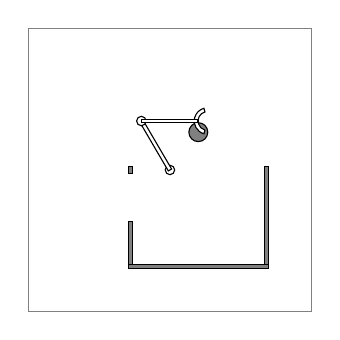
\begin{tikzpicture}
\begin{scope}[scale=1.2]
% bounding rect
\draw[color=black!50, thin] (-1.5,-1.5) rectangle (1.5,1.5);
\tikzstyle{dstyle}=[draw=black,fill=black!50]
\draw[dstyle] (0.300000,0.400000) circle (0.100000);
\draw[dstyle, shift={(0.300000,-1.020000)}, rotate=0.000000] (-0.740000,-0.020000) rectangle (0.740000,0.020000);
\draw[dstyle, shift={(1.020000,-0.480000)}, rotate=0.000000] (-0.020000,-0.520000) rectangle (0.020000,0.520000);
\draw[dstyle, shift={(-0.420000,-0.775000)}, rotate=0.000000] (-0.020000,-0.225000) rectangle (0.020000,0.225000);
\draw[dstyle, shift={(-0.420000,0.000000)}, rotate=0.000000] (-0.020000,-0.040000) rectangle (0.020000,0.040000);

\tikzstyle{dstyle}=[draw=black,fill=white]
\draw[dstyle] (0.000000,0.000000) circle (0.050000);
\draw[dstyle, shift={(-0.151454,0.258963)}, rotate=120.321137] (-0.300000,-0.020000) rectangle (0.300000,0.020000);
\draw[dstyle] (-0.302908,0.517926) circle (0.050000);
\draw[dstyle, shift={(0.397092,0.517926)}, rotate=180.000000](-74.484513:0.100000) arc (-74.484513:74.484513:0.100000) --(74.484513:0.140000) arc (74.484513:-74.484513:0.140000) -- cycle;
\draw[dstyle, shift={(-0.002908,0.517926)}, rotate=0.000000] (-0.300000,-0.020000) rectangle (0.300000,0.020000);

\end{scope}
\end{tikzpicture}
\caption{Invalid configuration}
\end{subfigure}%
\caption{Illustration of solution.}
\end{figure}

If we put some text in here, it shows up in the right place.

\begin{itemize}
\item comes from structure of multi-step problem
\item different cfrees
\item but they're very related!
\item inclusions, intersections
\end{itemize}

See Figure~\ref{fig:multi-space-example} for a simple motivating example.

\begin{figure}
\centering
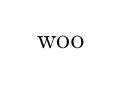
\begin{tikzpicture}

\node (a) at (0,0) {woo};

\end{tikzpicture}
\caption{An example of different $C_{free}$s}
\label{fig:multi-space-example}
\end{figure}

\subsection{Multiple sub-queries}

\subsection{Shared C-space}

\subsection{Each in a different C-free}

\subsection{Relations between C-frees (inclusion, intersection)}

\section{Related Work}

Jaillet and Simeon,
\emph{A PRM-based motion planner for dynamically changing environments}
\cite{jaillet2004dynamicprm}.
Explicit dichotomy between static and dynamic parts of the world.
Edges are checked when needed against moving obstacles;
their free-ness with respect to each is cached for the last tested position
for each obstacle.

Gayle, Klingler, and Xavier,
\emph{Lazy Reconfiguration Forest}
\cite{gayle2007lazyreconfigforest}.

Li and Shie,
\emph{An incremental learning approach to motion planning with
      roadmap management}
\cite{li2002incrementalprmmanagement}.
This is the Reconfigurable Random Forest (RRF).
They do ``roadmap management'' to handle changing environments,
and talk about doing some simple bounding-box stuff.

Lien and Lu,
\emph{Planning motion in environments with similar obstacles}
\cite{lien2009similarobstacles}.
This builds a PRM around obstacles in a database,
and then reposes them in a new world.

\section{Multi-Space Problem Definition}

Define the general problem.
Several spaces, each with a different checker.
Each checker has a different cost.

\section{Manipulation Examples of Multi-Space Problems}

\subsection{Multi-Step Problems (Moveable Obstacles)}

For segmented/labeled objects, we can automatically discover
different $C_{free}$s.
For example, we have an OpenRAVE module
which auto-discovers stuff.

Special case of this is if objects are disappearing.

\subsection{Changing Worlds (Broad-Phase Integration)}

relation to occupancy grid representations of workspace
(for deltas, conservative approxs, etc)

\subsection{Cached Self-Collision Checked Graphs}

\subsection{Padded Robots (Broad-Phase Integration)}

\subsection{Conservative Bounding Volumes for Different Grasps}

\subsection{Conservative Bounding Volumes for Hypothesized Objects}

\subsection{Dual Arm Stuff}

I think this is related.


\newpage
\chapter{Applying GreedyPRM to MultiSpace: the GreedyMultiPRM}

\begin{itemize}
\item GreedyPRM and multi-space are complementary
\item Apply greeydprm to multi-space problem
\item one planner that learns, can answer arbitrary queries
   in multiple related spaces faster and faster
\end{itemize}


\newpage
\chapter{A simple task planner using the GreedyMultiPRM}

\begin{itemize}
\item with/without inter-step relations
\item with/without padding
\item with/without self-checked cache
\item with/without relations for changing worlds
\item with/without conservative boxes for grabbed objects
\item constraints:
   \begin{itemize}
   \item handle with separate planner
   \item handle with relaxed constraint, followed by local optimizer
   \end{itemize}
\item run optimizer on paths occasionally and/or before executing
\end{itemize}

Also, there are incremental E-graphs \cite{phillips2013anytimeegraphs}
that we should relate the planner to and compare with.


\newpage
\chapter{Conclusion}

meta-graph [future work: probabalistic models]


\newpage
\chapter[Summary of Proposed Work]{Summary of\\Proposed Work}

\section{Timeline}

See Table~\ref{table:timeline} for the timeline.

\begin{table}
\centering
\begin{tabular}{lll}
\hline
Topic & Section & Deadline \\
\hline
Proposal & & January 2015 \\
Greedy PRM, Multi-Space & & January 2015 (RSS) \\
Cached Self-Collision Checked Graphs & & March 2015 (IROS) \\
?? & & June 2015 (Humanoids) \\
?? & & October 2015 (ICRA) \\
Writing & & November 2015 \\
Defence & & December 2015 \\
\hline
\end{tabular}
\caption{Proposed Timeline}
\label{table:timeline}
\end{table}


{\small
\bibliographystyle{abbrv}
\bibliography{pr-refs,siddpubs/siddpubs-conf,siddpubs/siddpubs-journal,siddpubs/siddpubs-misc}
}

\appendix
\chapter{Graph Search Proofs}
\label{appendix:gs-proofs}

This appendix presents some proofs relating the path-centric treatment
of graph search from Chapter~\ref{chap:inflate}
to traditional algorithms (e.g. A$^*$).

\begin{invariant}
The optimistically optimal path $path^* = A_s(G)$ can always be
segmented into
(a) a first sequence comprised of zero or more evaluated edges,
followed by
(b) a second sequence comprised of zero or more non-evaluated edges.
\label{inv:path-segmentation}
\end{invariant}

\begin{theorem}
Invariant~\ref{inv:path-segmentation} holds throughout the course of
$E_s$ [forward] (Algorithm~\ref{alg:e-s-forward}).
\label{thm:seg-fwd}
\end{theorem}

\begin{proof}
At the first iteration, with no edges evaluated,
$path^*$ will contain only non-evaluated edges,
and the invariant trivially holds.

Consider the case where the invariant newly does not hold for $path^*$.
In this case, there exists at least one triple of adjacent vertices
on the path $v_a, v_b, v_c$
such that the edge $(v_a, v_b)$ is un-evaluated,
while the edge $(v_b, v_c)$ has been evaluated.
Due to our invariant,
there must have been some previous iteration which returned a
$path'^*$ which contained the triple
$v'_a, v_b, v_c$ for some other $v'_a$,
with $(v'_a, v_b)$ evaluated.
Therefore, the shortest distance to $v_b$ must known (and can be
reached through $v'_a$),
and any subsequent optimistic-optimal path through $v_b$
must consist of only evaluated segments until $v_b$
(due to the way $A_s$ breaks ties).
But our current $path^*$'s segment $(v_a, v_b)$ is un-evaluated!
This contradiction shows that the invariant must hold throughout the
algorithm.
\end{proof}

\end{document}
